% =============================================================================================
% MD6329 final report, v1 (2026-10-24). Format: NeurIPS 2026 template (neurips_2026.sty, preprint option).
% Source of truth = this file + sections/*.tex. For Overleaf, upload overleaf.zip (single-file build of this
% document, made by build_overleaf.py) as a new project; compiler pdfLaTeX.
% Colours: \pending{} = repeat-0-only or draft content; \todo{} = still to write.
% =============================================================================================
\documentclass{article}

% numeric, compressed citations; must come before loading neurips_2026
\PassOptionsToPackage{numbers, compress}{natbib}

% "preprint": non-anonymous, no line numbers (a course report, not a NeurIPS submission)
\usepackage[preprint]{neurips_2026}

\usepackage[utf8]{inputenc} % allow utf-8 input
\usepackage[T1]{fontenc}    % use 8-bit T1 fonts
\usepackage{hyperref}       % hyperlinks
\usepackage{url}            % simple URL typesetting
\usepackage{booktabs}       % professional-quality tables
\usepackage{amsfonts}       % blackboard math symbols
\usepackage{nicefrac}       % compact symbols for 1/2, etc.
\usepackage{microtype}      % microtypography
\usepackage{xcolor}         % colors
\usepackage{amsmath,amssymb}
\usepackage{graphicx}
\usepackage{enumitem}
\usepackage[section]{placeins} % floats never drift past their section
\graphicspath{{figs/}}
\newcommand{\pending}[1]{\textcolor{orange}{#1}}
\newcommand{\todo}[1]{\textcolor{red}{[TODO: #1]}}
% GitHub account: change only these two lines
\newcommand{\repourl}{https://github.com/FelicityT1998/md6329-check-tha}
\newcommand{\demourl}{https://felicityt1998.github.io/md6329-check-tha/}
\title{Seeing Surgery Coming: Pixel-Supervised Multimodal Prediction of\\ 10-Year Hip Replacement in the CHECK Study}

\author{%
  Tian Fengxiao \\
  Student ID: G2606127G \\
  MD6329, Nanyang Technological University \\
  \texttt{FTIAN002@e.ntu.edu.sg}
}

\begin{document}
\maketitle

\begin{abstract}
Implants now last decades. For a 45--65-year-old with early hip complaints, the clinical question is therefore not only
whether OA is present but whether this hip will need replacing within the next ten years. We study this question in the
CHECK study (1,002 participants, 1,705 hips, 93 replacements within ten years), using only information available at the
first consultation. A penalised logistic model on examination and symptoms reaches AUPRC 0.37 (AUROC 0.81). Tree
ensembles and an FT-Transformer do not improve on it, although the transformer adds better calibration and 2/5-year risk.
Frozen ImageNet features of the baseline radiograph add nothing. A small residual head on frozen DenseNet feature maps,
supervised with OARSI reading items used only as training targets, extracts substantial pixel signal. Its cross-fitted
logit lifts the clinical model to AUPRC 0.55 and AUROC 0.89 in internal nested cross-validation ($\Delta$AUPRC $+0.20$,
95\% CI 0.12--0.29); no external cohort was available. The gain persists after events in the first two years are
excluded. A temporal audit, shortcut probes and pseudo-external
validation show that discrimination transports across centres but calibration does not.
\end{abstract}

% =============================================================================================
% 1 Introduction (problem formulation + related work)
% Numbers: 实验结果汇总.md (5-repeat run, 2026-10-24); literature: litreview/abstracts.md
% =============================================================================================
\section{Introduction}
\label{sec:intro}

\paragraph{The clinical problem.}
Hip osteoarthritis (OA) has no single diagnostic standard. The clinical criteria of the American College of Rheumatology
rest on hip pain, restricted internal rotation and morning stiffness~\cite{altman1991acr}; NICE allows a diagnosis without
imaging~\cite{nice2022oa}; epidemiology relies on the radiographic Kellgren--Lawrence (KL) grade and the OARSI atlas
items~\cite{altman2007oarsi}. The three often disagree: among early symptomatic patients, radiographic OA is almost as
common in painless as in painful hips~\cite{rondas2022}. For the end stage, total hip arthroplasty (THA) is
effective, and implants now last: about 58\% of hip replacements still function after 25 years~\cite{evans2019hip}.
This shifts the clinical question for the 45--65-year-old patient. Every year of joint survival counts, because a younger
recipient carries a higher lifetime risk of revision~\cite{bayliss2017revision}. What guides the intensity of conservative
care, the timing of orthopaedic referral and the enrolment in joint-preserving trials is therefore a \emph{long-horizon}
estimate of whether, and roughly when, this hip will need replacing.

\paragraph{What AI prediction offers so far.}
Prediction work in OA is dominated by the knee, and the hip makes up only 8--15\% of OA--AI studies~\cite{binvignat2022}.
Most hip models classify the current KL grade or predict incident radiographic OA. Only one large study predicts THA
from pixels: in the Osteoarthritis Initiative (OAI) a model with deep-learning radiographic measurements reached AUROC
0.81 and AUPRC 0.28 for 10-year THA at a 2.4\% event rate~\cite{jang2023}. External validation remains rare. When it is
done, performance falls; for example, a seven-cohort hip model dropped from AUROC 0.81 to 0.64 under leave-one-cohort-out
validation~\cite{vandenberg2026}. Table~\ref{tab:forest} summarises the prognostic literature. The \textbf{Cohort Hip and
Cohort Knee (CHECK) study} is the natural test bed for the surgical question~\cite{wesseling2016}. Between 2002 and 2005,
ten Dutch hospitals enrolled 1,002 people aged 45--65 with hip or knee pain, at or within six months of their first
general-practitioner visit for these symptoms; participants were referred by general practitioners or responded to
advertisements. They were followed for ten years with
questionnaires, standardised examination and radiographs. In our analysis this gives 2,004 hips; 1,705 have known 10-year
status, and 93 (5.5\%, in 75 people) were replaced. We use every baseline item that is fixed at first presentation: 76
clinical features in six groups and the pixels of the baseline anteroposterior (AP) pelvic radiograph. Linear, tree and
FT-Transformer models handle the tables. A supervised residual head on frozen DenseNet features turns the pixels into a
single risk score, and an elastic net fuses the two.

\begin{table}[!tbp]
  \centering
  \caption{\textbf{Prognostic models for hip (and, for reference, knee) OA: cohort, event rate and performance.}
  Left: discrimination (AUROC; solid bars = reported 95\% CI, dashed = Hanley--McNeil interval from hips and events, or
  $\pm$SD across held-out cohorts; marker area $\propto\log$ events). Right: AUPRC divided by the event rate, the only
  scale on which precision is comparable across cohorts; studies that do not report the event rate show the raw AUPRC.
  Colours give the model input. Endpoints differ (THA, radiographic OA (rHOA), KL progression), so no pooled estimate is
  drawn. Our rows (grey band) are nested cross-validation means; CIs from a participant-clustered bootstrap. Agricola
  2013 reports apparent performance (shape modes selected and evaluated on the same data).}
  \label{tab:forest}
  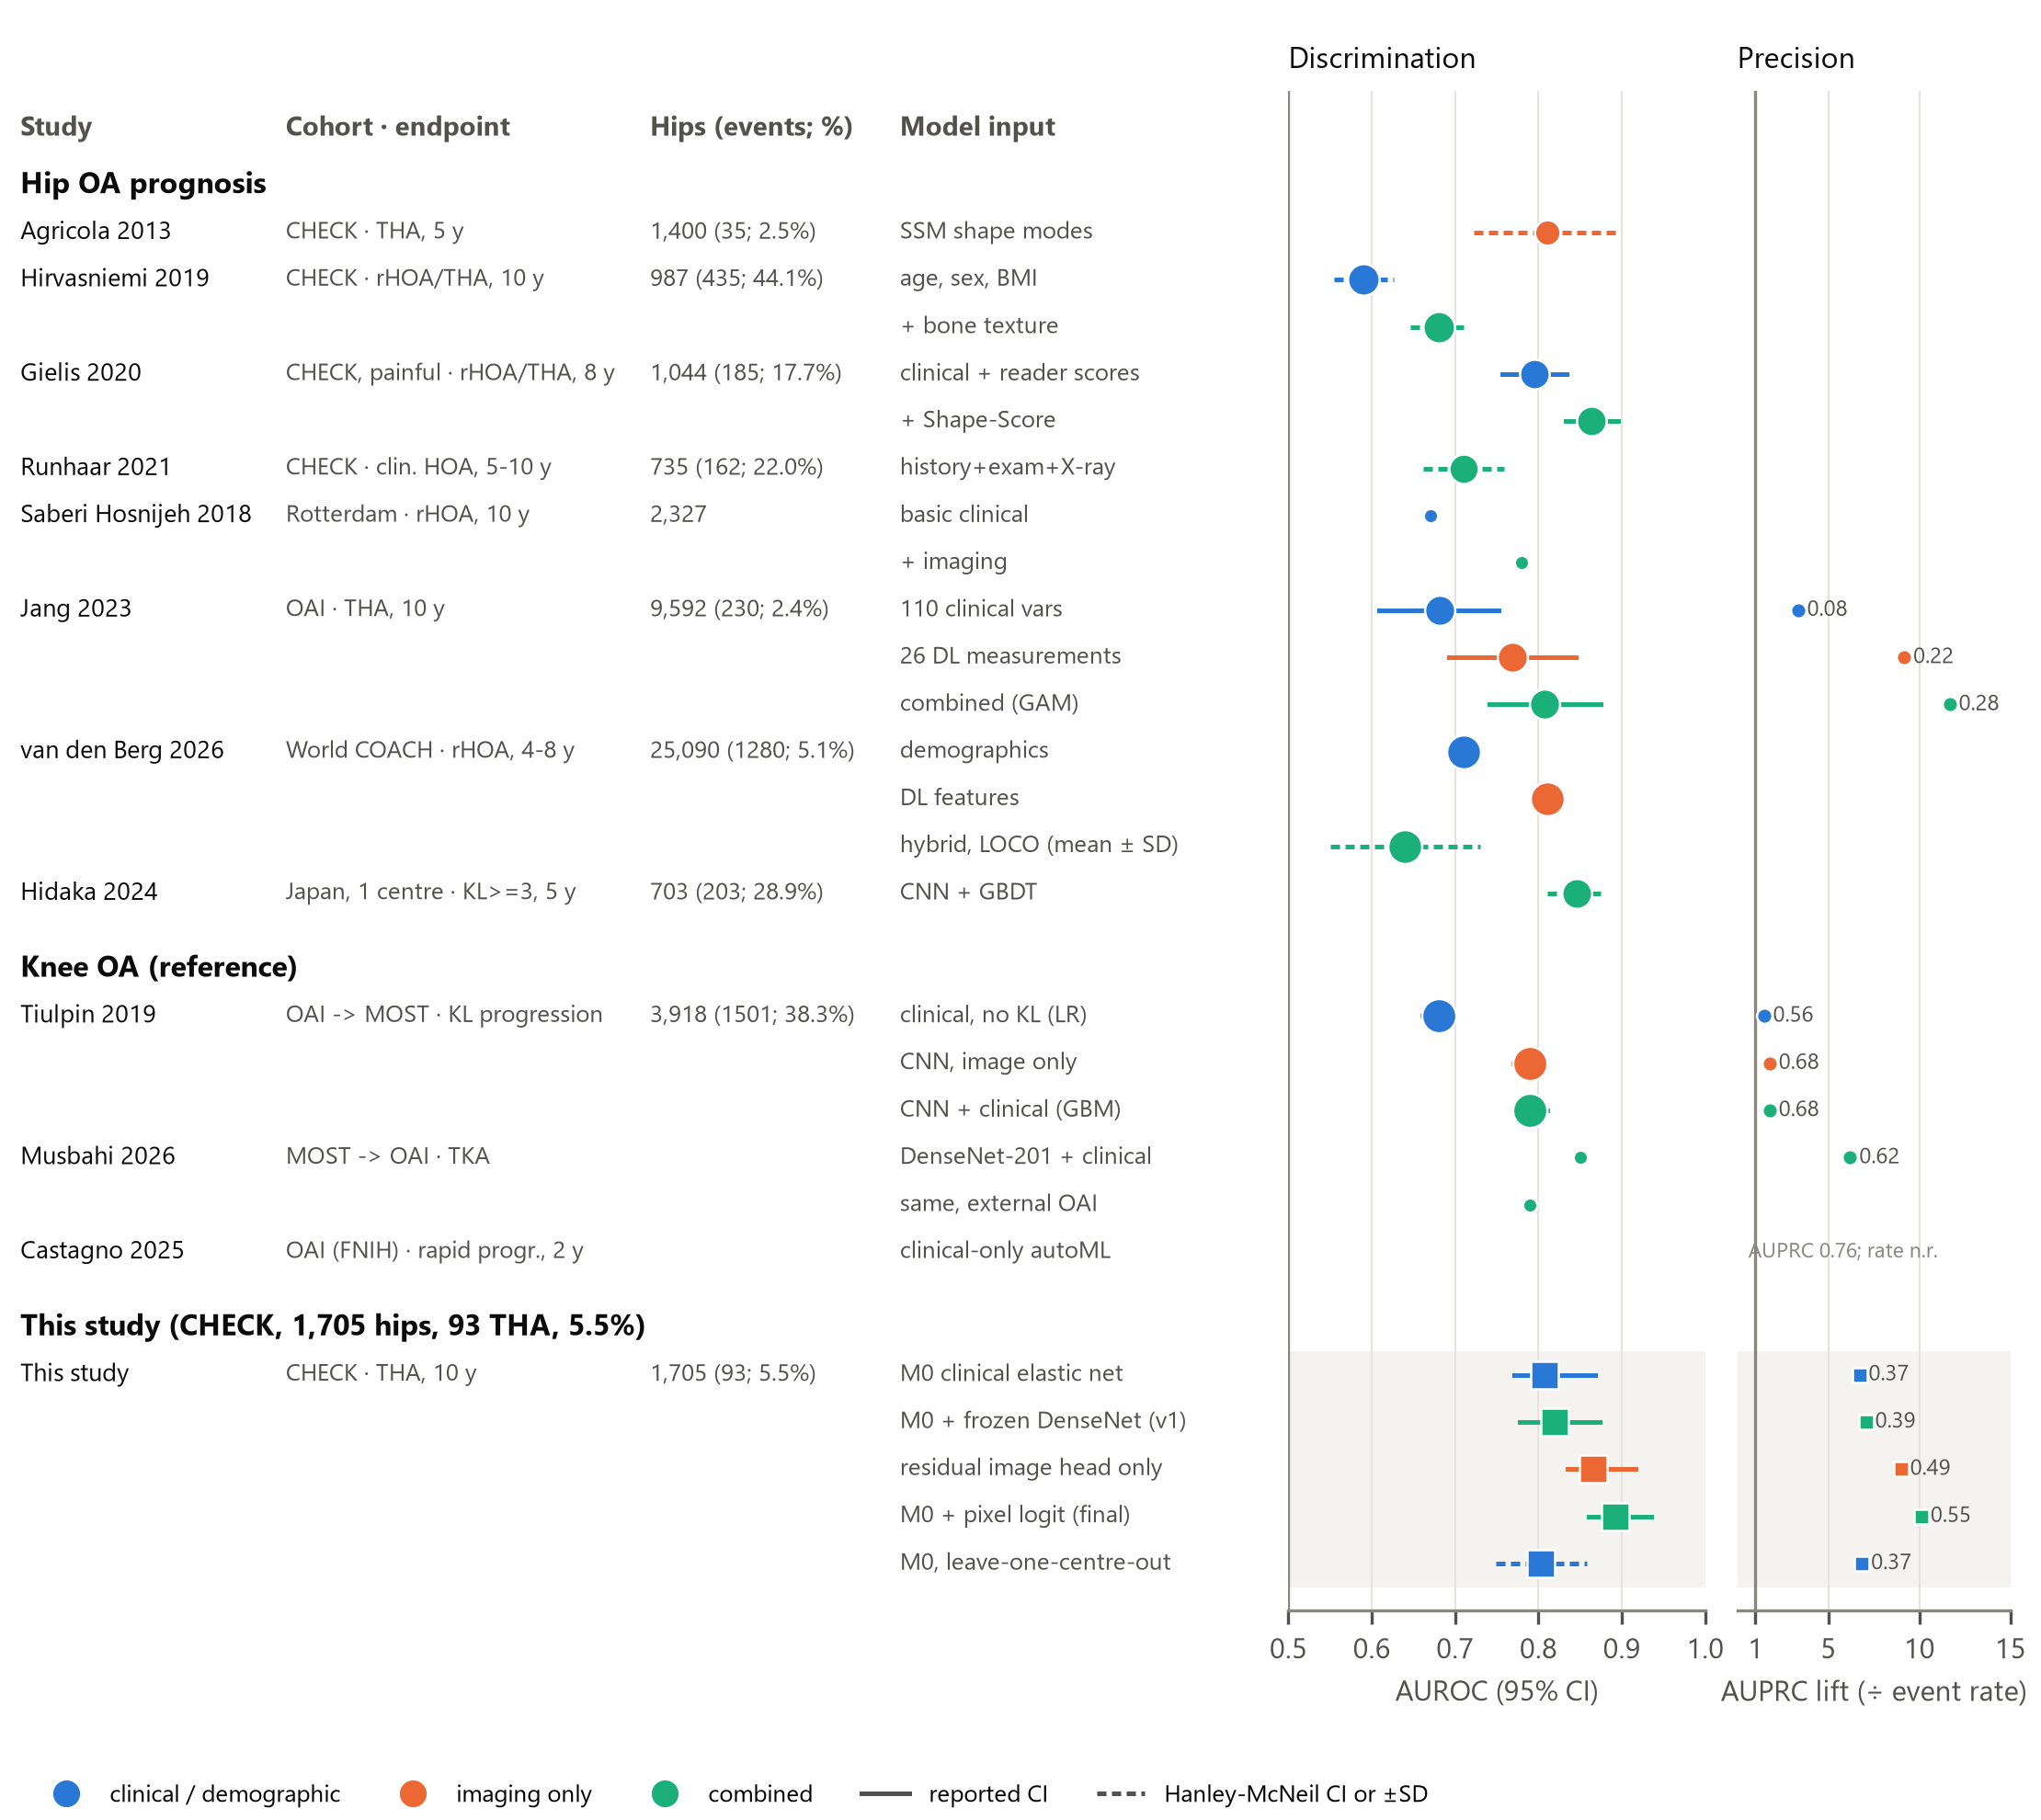
\includegraphics[width=\linewidth]{tab1_forest.png}
\end{table}

\paragraph{Prior work on CHECK and on the knee.}
Hip models built on CHECK share a pattern~(Table~\ref{tab:forest}). The image enters as hand-crafted structure:
statistical shape modes predict 5-year THA (AUROC 0.81, 35 events)~\cite{agricola2013}, an automated Shape-Score raises
8-year radiographic OA prediction from 0.795 to 0.864~\cite{gielis2020}, and bone texture adds 0.09 to a demographic
model~\cite{hirvasniemi2019}. The endpoints are mostly radiographic. Several models also contain the baseline KL grade,
which in the public CHECK release was read after follow-up, paired with later films~\cite{macri2022}. Clinical-only
predictors are weak for radiographic outcomes~\cite{saberihosnijeh2018,vanberkel2021}. For arthroplasty, however,
symptoms (WOMAC), age and sex are the established predictors~\cite{zarringam2020}. The surgical endpoint is thus where
non-imaging information should be given importance.

\paragraph{}
Knee studies show what changes with anatomy and endpoint. On standing knee films the joint space is seen directly,
without pelvic overlap, and the outcome (KL progression) is itself read from the film. So an end-to-end CNN with a KL
auxiliary task beats clinical data (0.79 vs 0.68)~\cite{tiulpin2019}. For surgery, a DenseNet with clinical inputs
reaches 0.85 internally and 0.79 externally~\cite{musbahi2026}. Clinical-only models transport well~\cite{castagno2025}.
A systematic review of 33 deep-learning studies found that combining imaging modalities did not consistently help, that
external validation lowered the median AUC from 0.81 to 0.75, and that surgical endpoints also reflect access to
care~\cite{gillani2026}. The hip joint is deep,
small on a pelvic film, and partly hidden by the acetabular rim. Its early signs (superolateral joint-space narrowing,
marginal osteophytes) are millimetre-scale and local. A frozen, globally pooled ImageNet embedding is therefore unlikely
to capture them.

\paragraph{Connection to the course.}
Our image baseline follows the frozen-feature-extractor approach of Bar et al.\ (Lecture 2, slides 102 and 126--127;
video 1:00--1:05). The decision to freeze rather than fine-tune follows the transfer-learning guidance for scarce
labelled data (Lecture 2, slides 106--114; video 0:54--0:56). DenseNet-121 is the CheXNet backbone, whose saliency maps
motivated our attention maps (Lecture 2, slide 158; video 1:29--1:31). Class-weighted losses for imbalance follow
Lecture 3 (slides 63--64; video 0:31--0:34). Our token, FiLM and logit fusions map onto the early, joint and late fusion
types of Lecture 8 (slide 30; video 0:11--0:14), and our SimCLR pretraining onto its self-supervision section (slides
42--50; video 0:17--0:20). Appendix~\ref{app:lectures} lists all links.

\paragraph{}
Our design follows from these observations. (i) With 93 events and 76 features (about 1.2 events per feature), a
penalised linear model is the reference that every deep model must beat~\cite{christodoulou2019}. (ii) The image head
keeps the $14\times14$ spatial map of a frozen DenseNet-121 and adds two residual blocks with attention pooling. Its
features are supervised with the 11 OARSI reading items, used \emph{only as training targets}, so the future-informed
readings never become predictors. (iii) The image enters the clinical model as one cross-fitted logit, a learned
analogue of Jang's measurements~\cite{jang2023}, because token fusion overfits at this sample size. (iv) No external
cohort with the same inputs was available. Every estimate is therefore internal (nested cross-validation within CHECK),
and transportability is probed with pseudo-external splits across centres, film formats and patient subgroups rather
than claimed.

\paragraph{Research question and clinical setting.}
We fix the prediction time $t_0$ at the first consultation for hip or knee complaints, when the AP pelvic radiograph is
taken. The question is: \emph{from history, questionnaires, a standardised hip examination and the raw pixels of that
same-day radiograph (with no radiologist's grading and no research biomarkers), what is this hip's risk of replacement
within ten years?} The intended uses are deciding how intensive conservative management should be and how often to
review, timing the referral to an orthopaedic surgeon, and enriching joint-preservation trials with high-risk hips. Two
uses are excluded. Hips that are already on a surgical pathway at $t_0$ gain nothing from prediction. Population-level
planning is also out of scope without local recalibration (Section~\ref{sec:res-aux}). We ask four things:
\begin{enumerate}[leftmargin=*,itemsep=0pt,topsep=2pt]
  \item How much do examination and symptoms add beyond demographics?
  \item Does a deep tabular model outperform a penalised linear model?
  \item Can radiographic signal be extracted from pixels alone, without readings at prediction time?
  \item Do discrimination and calibration transport across centres, film formats and patient subgroups?
\end{enumerate}
Figure~\ref{fig:overview} summarises the inputs, models and outputs of the study.

\begin{figure}[!tbp]
  \centering
  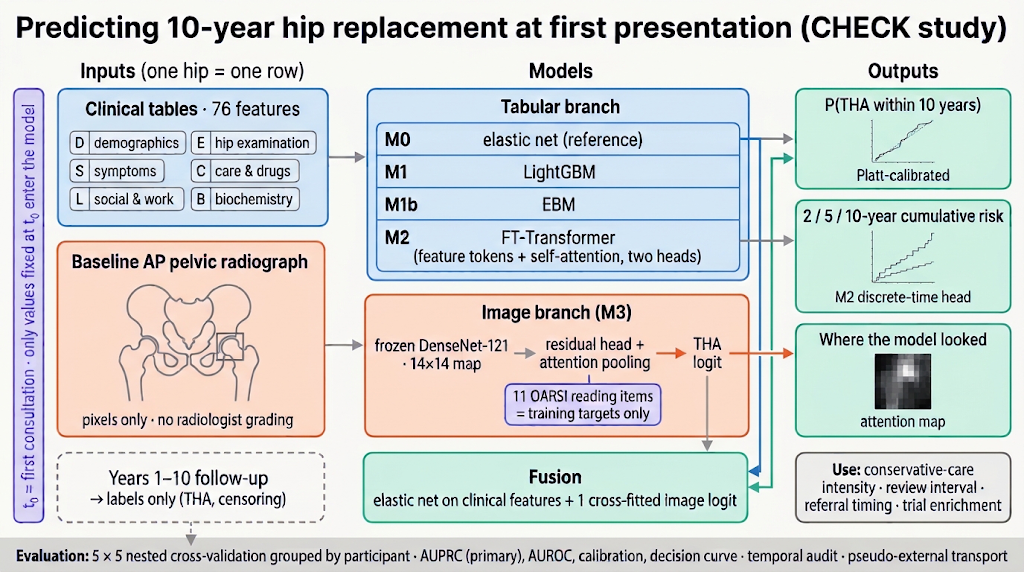
\includegraphics[width=\linewidth]{fig1_overview.png}
  \caption{\textbf{Inputs, models and outputs.} Baseline clinical tables (76 features, groups D/E/S/C/L/B) and the
  baseline AP pelvic film are the only inputs. The tabular branch compares a penalised linear model with tree ensembles
  and an FT-Transformer. The image branch converts each hip crop into one THA logit. The final model is an elastic net on
  clinical features plus that logit. Outputs are the Platt-calibrated 10-year THA probability and, from the
  FT-Transformer's discrete-time head, 2/5/10-year cumulative risk.}
  \label{fig:overview}
\end{figure}

% =============================================================================================
% 2 Methods. Each paragraph <= 100 words (user constraint).
% v2 (2026-10-24 evening): EDA rewritten as findings -> design; timeline figure moved here; M0 figure added;
% contralateral-information statement added to the pipeline paragraph.
% =============================================================================================
\section{Methods}
\label{sec:methods}

\paragraph{Overall design.}
The unit of analysis is the hip; resampling is by participant. The outcome is ipsilateral THA within ten years. It is
defined by the prosthesis flag, the first post-operative visit, or a prosthesis recorded on a follow-up film. The reading
file stores the last case as code 5 in the KL field. This is not a KL grade (KL ends at 4); it never occurs at baseline,
and 89 of the 91 hips with this code are replaced hips. Every disagreement was checked against the films. Clinical tables feed M0 (elastic net), M1 (LightGBM), M1b (EBM) and M2 (FT-Transformer). The
radiograph feeds M3, a supervised image head, and the fusion model gives M0 the cross-fitted M3 logit
(Fig.~\ref{fig:overview}). Estimates come from 5$\times$5 nested cross-validation (CV), with AUPRC as the primary metric.
Figure~\ref{fig:timeline} places every input and label on the study timeline.

\begin{figure}[!tbp]
  \centering
  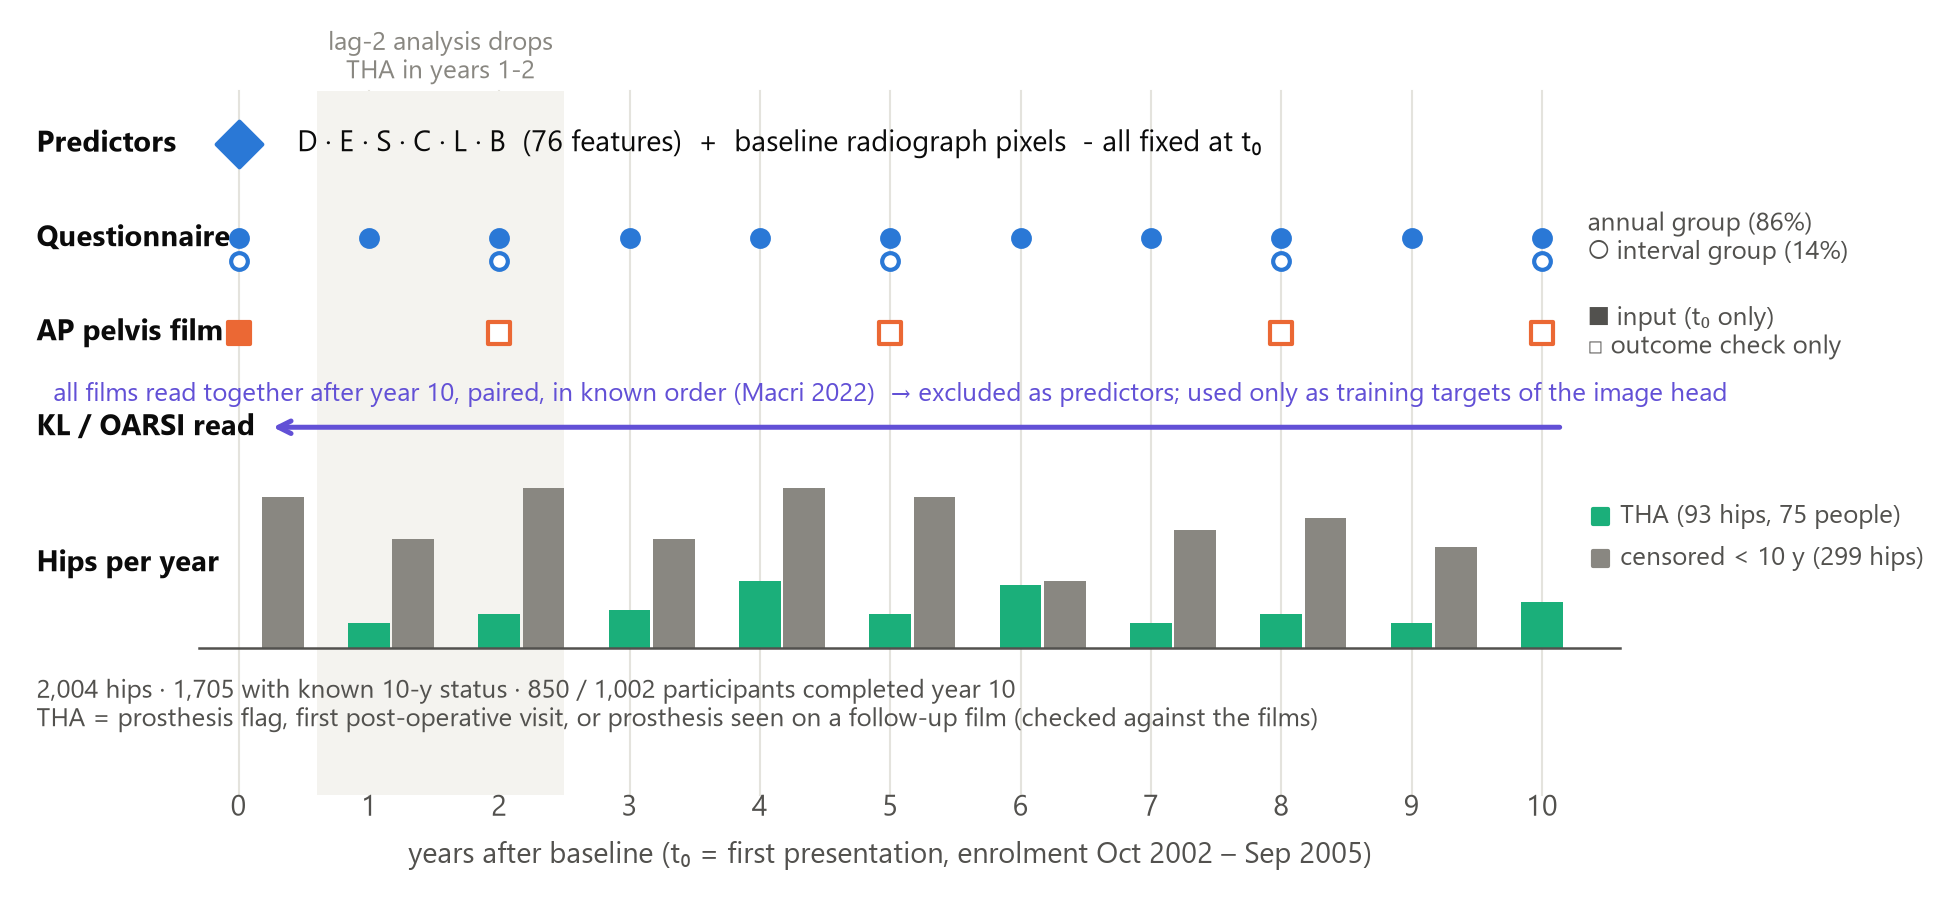
\includegraphics[width=\linewidth]{fig2_timeline.png}
  \caption{\textbf{Study timeline and the admissibility of each input.} Predictors are restricted to values fixed at
  $t_0$: the six clinical feature groups and the baseline AP pelvic film. Later questionnaires and films serve only to
  define THA and censoring. The public KL/OARSI readings were scored after year 10 with all films side by
  side~\cite{macri2022}; they are therefore excluded as predictors and used only as training targets of the image head.
  Bars show THA (green) and censoring before year 10 (grey) per year; 152 of 1,002 participants did not complete year 10
  (older, more often not in paid work; standardised mean differences $\le0.18$). The shaded band marks the events
  removed in the lag-2 analysis.}
  \label{fig:timeline}
\end{figure}

\paragraph{Exploratory analysis: cohort and outcome.}
No exploratory step used model fits. Of 2,004 hips, 1,705 have known 10-year status and 93 were replaced
(Fig.~\ref{fig:s-flow}); the Kaplan--Meier 10-year risk is 5.1\%. Risk differed sharply by ipsilateral hip pain (10.2\%
vs 1.7\%) and by internal rotation $\le25^\circ$ (10.5\% vs 2.7\%), but little by visiting group or film format
(Fig.~\ref{fig:s-km}). Across the ten recovered centres it ranged from 1.7\% to 7.9\% (Fig.~\ref{fig:s-km-centre};
participant-clustered GEE $p=0.36$). The two hips of a participant are dependent: a quarter of participants with one
THA also had the other hip replaced.

\paragraph{Exploratory analysis: examination and symptoms.}
Examination items were graded rather than threshold-like. Per standard deviation, internal-rotation ROM had univariable
OR 0.46 and flexion ROM 0.54; each grade of pain on internal rotation or flexion had OR 2.0 and 1.7. Contralateral
internal rotation still carried signal (OR 0.76). Dichotomising internal rotation at $25^\circ$ (OR 4.1) discards this
gradient. Ipsilateral hip pain was the strongest symptom (OR 6.0), WOMAC function and pain were weaker (1.4/SD), and
biomarkers were weak ($\le1.34$/SD). Ipsilateral knee pain had OR 0.43. This pattern marks ``bystander'' hips, which
were enrolled because of the knee.

\paragraph{Exploratory analysis: collinearity, missingness and distributions.}
Several inputs measure the same construct twice. Left and right ROM correlate at $\rho$ = 0.77--0.84, each ROM correlates
with its own cut-off ($\rho\approx-0.8$), current and weekly pain correlate at 0.83, and the WOMAC total is the exact sum
of its subscales. Within the examination block, VIF reached 6.1. Missingness followed three mechanisms
(Fig.~\ref{fig:s-missing}). Some items were gated by a complaint or status (38 raw variables). Some depended on the
centre protocol (41), with missing rates of 0 or 1 by centre. The rest were sporadic (2--5\%; 92). Fifteen continuous
variables had $|\text{skew}|>1$ (Fig.~\ref{fig:s-skew}).

\paragraph{How the exploratory analysis shaped the design.}
Three principles followed. First, the model should not depend on which member of a correlated pair it picks. M0
therefore uses an elastic-net penalty, whose $\ell_2$ part spreads weight across correlated features; inner tuning chose
ridge-dominant mixing ($\ell_1$ ratio 0.1--0.3) in 20 of 25 outer folds. Trees and the FT-Transformer handle correlation
natively. Second, when two inputs carry the same information, the one closer to clinical practice and easier to obtain
enters the model; the other is kept for reference. Third, no input may encode the centre through its missingness.

\paragraph{}
The second principle kept the continuous ROM and pain grades, with the $25^\circ$/$115^\circ$ cut-offs used only for
description. It kept the weekly pain score, which depends less on the visit day, and the WOMAC subscales rather than
their sum. Contralateral values enter as asymmetry terms (ipsilateral minus contralateral). Under the third principle,
external rotation, adduction and abduction ROM and the bursitis/tendinitis tests left the main set because of their
centre-specific missingness, not their signal; they enter sensitivity analyses only. The final set has 76 features,
maximum VIF 5.1, and three pairs with $|\rho|\ge0.7$ (Fig.~\ref{fig:corr}).

\begin{figure}[!tbp]
  \centering
  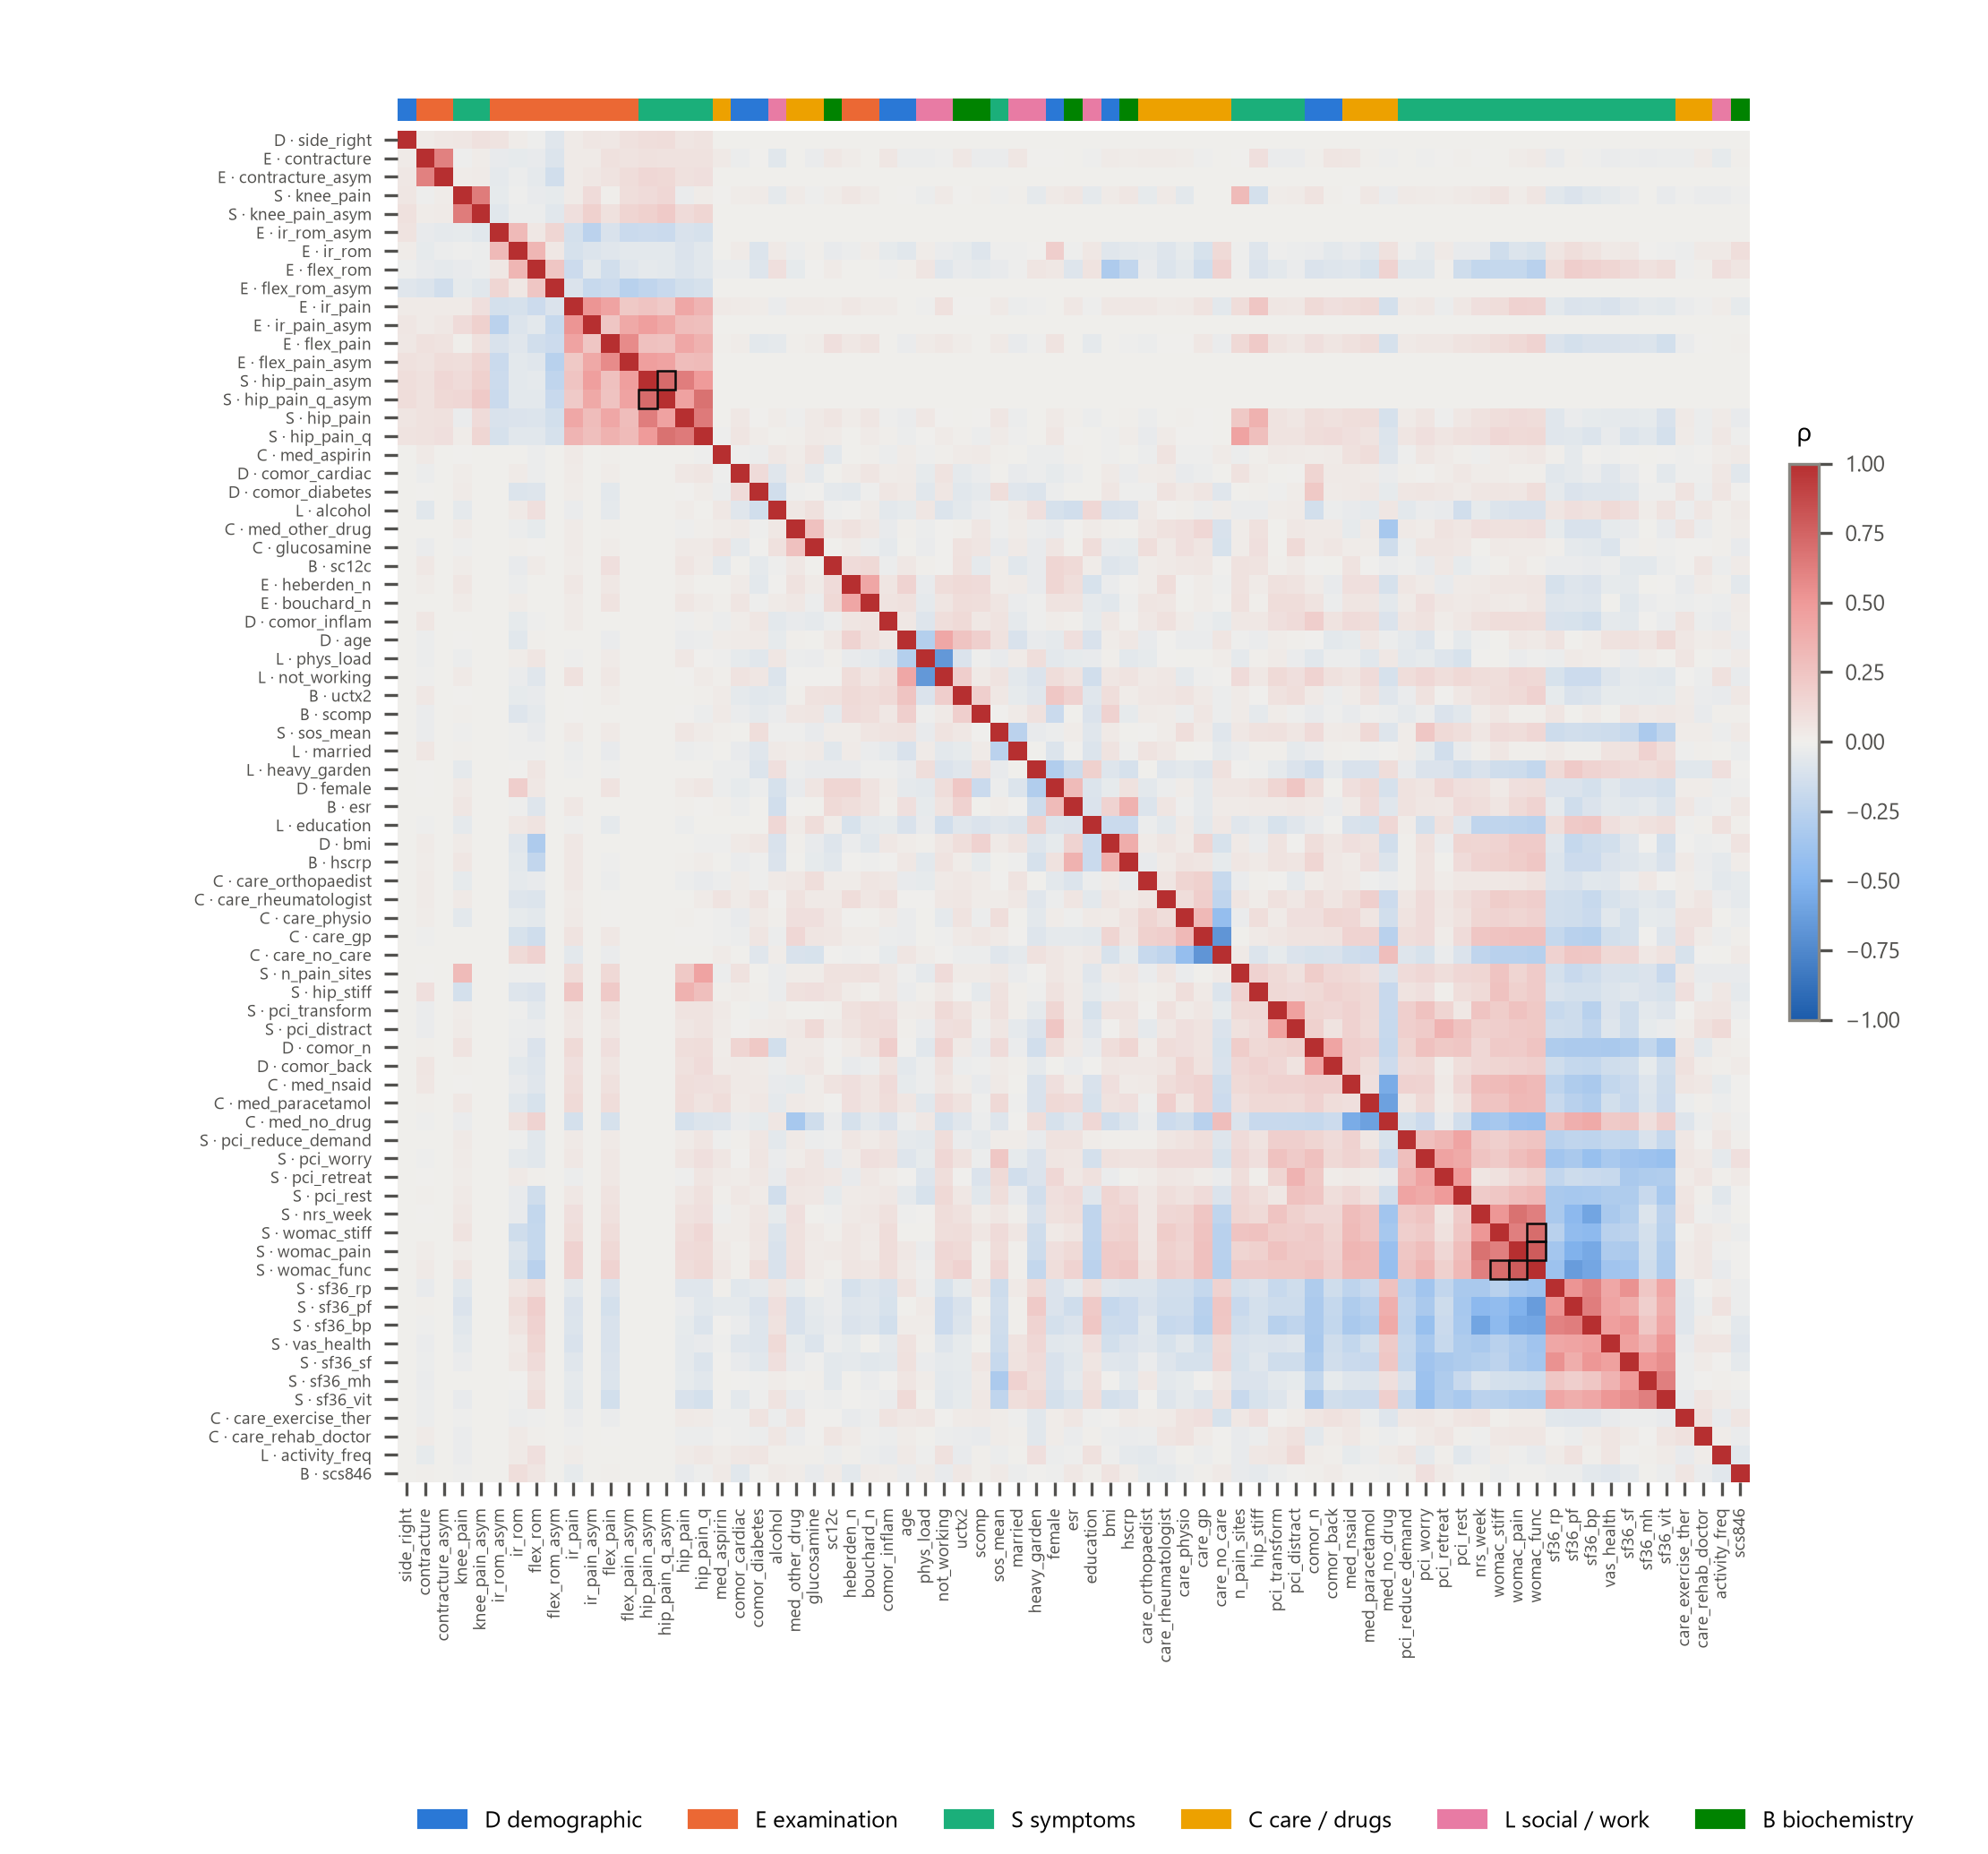
\includegraphics[width=0.92\linewidth]{fig3_correlation.png}
  \caption{\textbf{Spearman correlation of the 73 numeric main features} (three nominal features not shown), ordered
  by hierarchical clustering; the strip marks the feature group. Boxed cells: $|\rho|\ge0.7$, namely WOMAC
  pain--function (0.79), WOMAC stiffness--function (0.71) and the two hip-pain asymmetry terms (0.71). The symptom
  scales form one block. Hip-examination items cluster with ipsilateral hip pain, and SF-36 domains form an inverse block.}
  \label{fig:corr}
\end{figure}

\paragraph{Data partition and pipeline.}
Folds are stored once and shared by every model (Fig.~\ref{fig:pipeline}). The outer loop is 5-fold
StratifiedGroupKFold, repeated five times. It is grouped by participant and stratified by the participant's number of THAs
(0/1/2) $\times$ film format, which gives 17--20 events per test fold. Inside each outer training set, three
participant-grouped inner folds serve hyper-parameter selection, early stopping, Platt calibration and cross-fitting of
the image logit. We report the mean over repeats of each pooled out-of-fold metric. 95\% CIs (500 draws) and paired
differences ($\Delta$; 1,000 draws) come from a participant-clustered bootstrap of repeat~0.

\paragraph{No information from the other hip beyond baseline.}
A model scoring one hip sees the other hip only through $t_0$ values. Asymmetry terms are computed from the baseline
table. The image crop contains one hip, and the auxiliary reading targets are ipsilateral. The other hip's follow-up
data, including its THA, are never inputs. Both hips of a participant always fall in the same fold, so the other hip's
label cannot cross a train/test boundary. The participant's THA count is used only to stratify the folds. We verified
each of these points in the code.

\begin{figure}[!tbp]
  \centering
  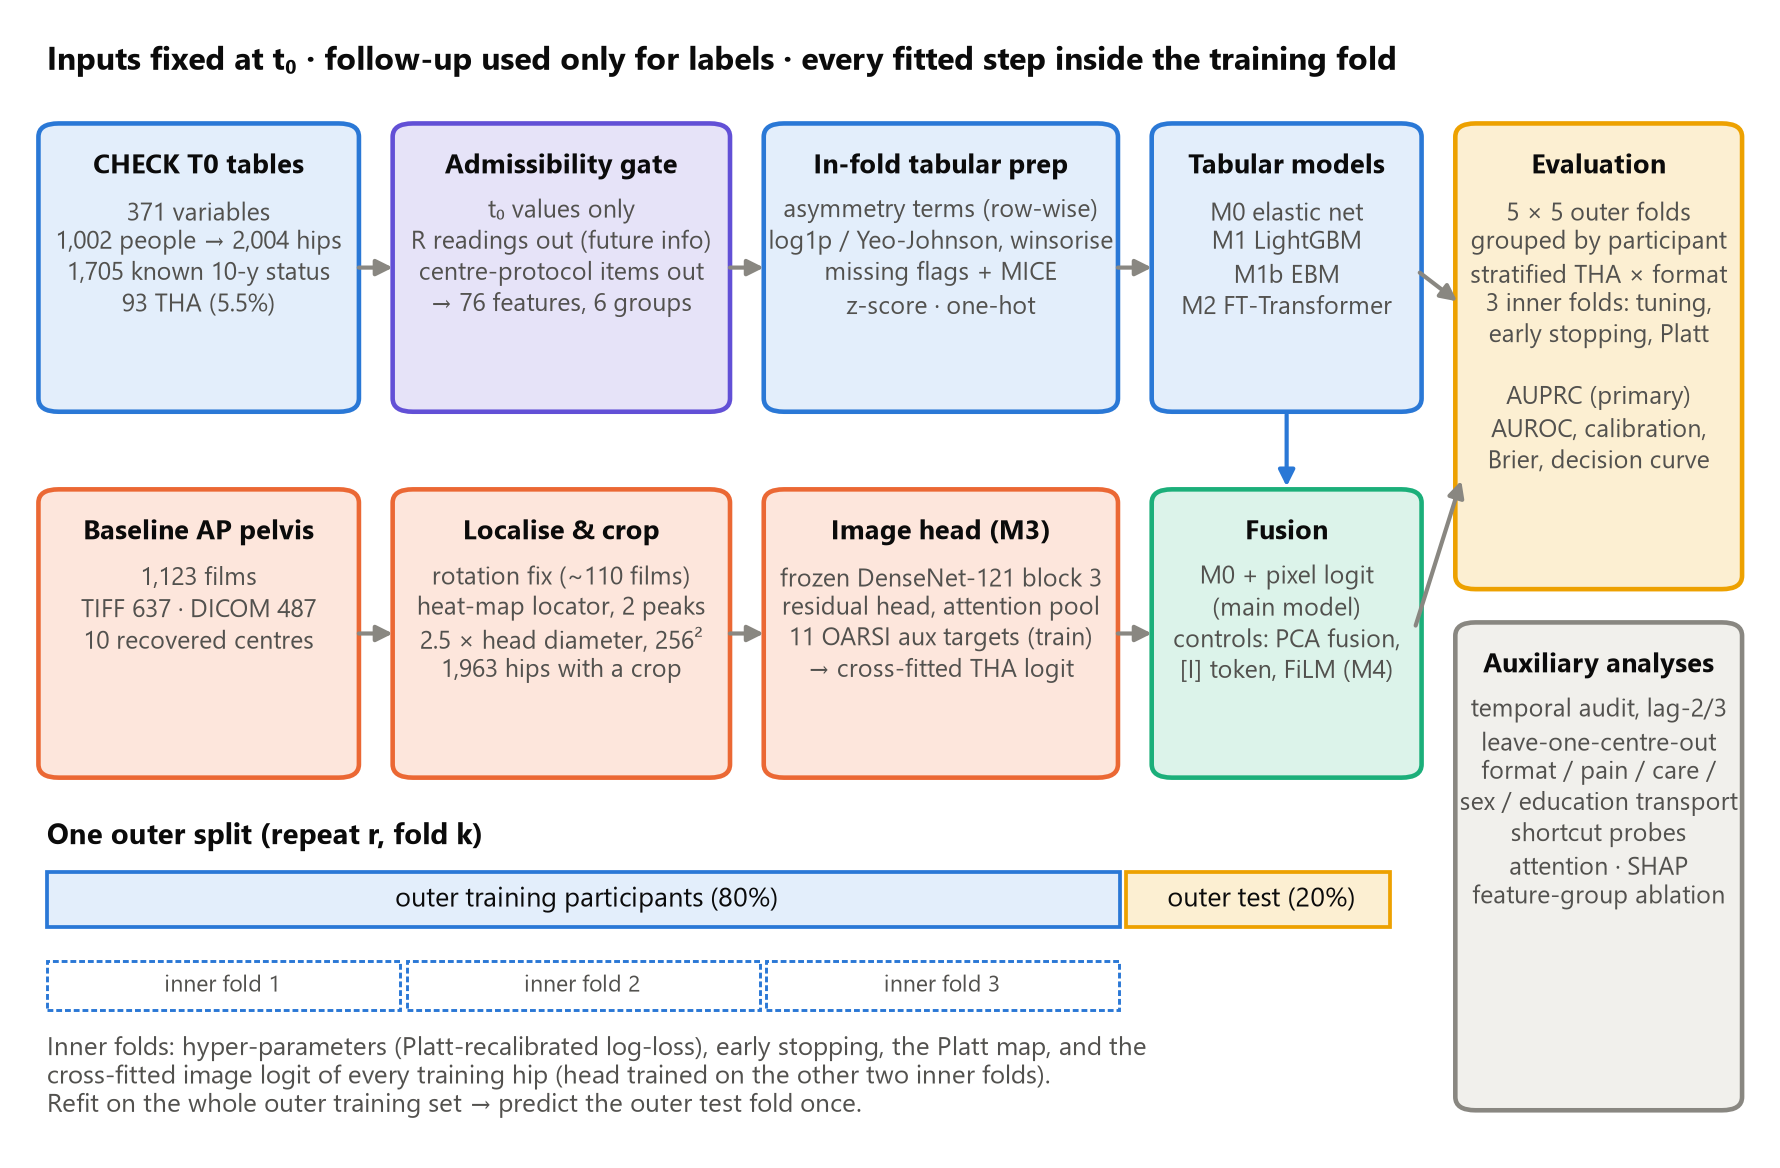
\includegraphics[width=\linewidth]{fig4_pipeline.png}
  \caption{\textbf{Pipeline and fold layout.} Inputs pass an admissibility gate (values fixed at $t_0$ only). Tabular
  preprocessing is fitted inside each training fold. The image path is reorientation, femoral-head localisation,
  cropping, frozen DenseNet features and the trainable head, whose logit is cross-fitted. Bottom: one outer split; the
  three inner folds are used for tuning, early stopping, Platt calibration and cross-fitting.}
  \label{fig:pipeline}
\end{figure}

\paragraph{Preprocessing without leakage.}
A line-by-line code audit confirmed that every fitted step runs on the current training rows only, in this order:
\begin{enumerate}[leftmargin=*,itemsep=0pt,topsep=2pt]
  \item row-wise asymmetry terms and structural rules (below);
  \item log1p for biomarkers and Yeo--Johnson for other variables with $|\text{skew}|>1$, both fitted on training rows
        (Fig.~\ref{fig:s-skew});
  \item winsorising at the training 0.5/99.5\% quantiles;
  \item missing indicators;
  \item MICE imputation of sporadic gaps (BayesianRidge, 10 rounds, outcome excluded);
  \item $z$-scoring and one-hot coding.
\end{enumerate}
Validation and test rows are only transformed. Trees keep NaN, and the FT-Transformer uses a learned per-feature [MISS]
token. Three label-free steps used all rows: the transform type per variable, the redundancy rules, and the
image-normalisation models below.

\paragraph{Structural rules.}
Gated items are not missing at random, so they were coded from the questionnaire logic (Fig.~\ref{fig:s-missing}). Hip
morning stiffness was asked only of participants who reported hip complaints: it is missing in 9\% of hips without hip
pain and in none with pain. A skipped item therefore means ``no hip complaint reported'' and is coded as no stiffness.
Physical workload was asked only of people in paid work, so non-workers receive the lowest level plus a not-working
indicator. Menopause has its own category for men. Missing categories get an indicator.

\paragraph{Image preprocessing and annotation.}
There were 1,123 baseline films (637 digitised-film TIFF scans, 487 DICOM). About 110 TIFF scans were stored rotated by
$90^\circ$. A self-supervised four-way rotation classifier (ResNet-18; 98.5\% accuracy on held-out rotations) restored
them. We annotated femoral-head centres and radii on 162 stratified films (279 heads) and trained a ResNet-18 U-net
heat-map locator on them. Decoding two peaks gave a median error of 0.27 head radii (3-fold subject CV). Crops measure
$2.5\times$ head diameter at $256^2$, 16 bit, with left hips mirrored. After visual QC, 1,963 hips have a crop,
including every THA hip.

\paragraph{Tabular models.}
M0, the reference and the clinical part of the final model, is an $\ell_1/\ell_2$-penalised logistic
regression~\cite{zou2005elasticnet} on the preprocessed features (Fig.~\ref{fig:m0}). Its 40 candidate configurations
span $C$ from $1.5\cdot10^{-3}$ to 9.6 (log scale), $\ell_1$ ratio from 0 to 1 and class weighting on or off. M1 is
LightGBM with depth-limited trees and class weights~\cite{ke2017lightgbm}. M1b is an explainable boosting
machine~\cite{nori2019interpretml}, the same model family as Jang's GAM~\cite{jang2023}.

\paragraph{}
We did not resample the data (no SMOTE), because imbalance correction does not improve discrimination and harms
calibration~\cite{vandengoorbergh2022}. We used class weights or focal loss instead, followed by Platt
recalibration~\cite{platt1999} fitted on inner out-of-fold predictions. All candidate configurations were drawn once
with a fixed seed, and every outer fold scores the same list.

\begin{figure}[!tbp]
  \centering
  \IfFileExists{figs/fig5_m0.png}{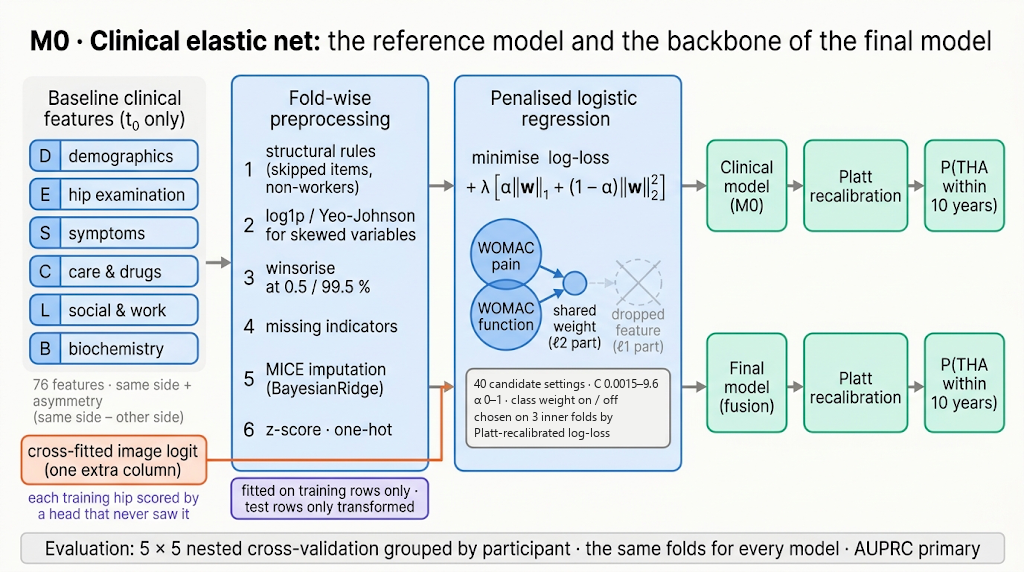
\includegraphics[width=\linewidth]{fig5_m0.png}}{%
    \fbox{\parbox[c][4cm][c]{0.95\linewidth}{\centering\todo{fig5\_m0.png: M0 diagram (Gemini prompt in figure\_prompts\_gemini.md)}}}}
  \caption{\textbf{M0 clinical elastic net and its use in the final model.} Raw baseline features pass the fold-wise
  preprocessing chain (asymmetry and structural rules, skew transforms, winsorising, MICE with missing indicators,
  $z$-scoring and one-hot coding). An $\ell_1/\ell_2$-penalised logistic regression, tuned on three inner folds by
  Platt-recalibrated log-loss, gives the clinical model. In the final model the same learner receives one extra column,
  the cross-fitted image logit, and its output is Platt-recalibrated.}
  \label{fig:m0}
\end{figure}

\paragraph{Feature engineering for the FT-Transformer.}
The FT-Transformer receives the same $z$-scored numerics (Fig.~\ref{fig:ftt}). Each feature $j$ becomes a $d$-dimensional
token,
\[
  t_j = \phi_j(x_j) + e_j + g_{\mathrm{group}(j)},
\]
where $\phi_j$ is a linear, periodic or piecewise-linear value embedding (bins from training quantiles), $e_j$ a learned
feature-ID embedding and $g$ a group embedding. Categorical features use embedding tables. A [CLS] token is prepended.
All three tokeniser types entered the architecture search; the selected architectures use the linear one.

\begin{figure}[!tbp]
  \centering
  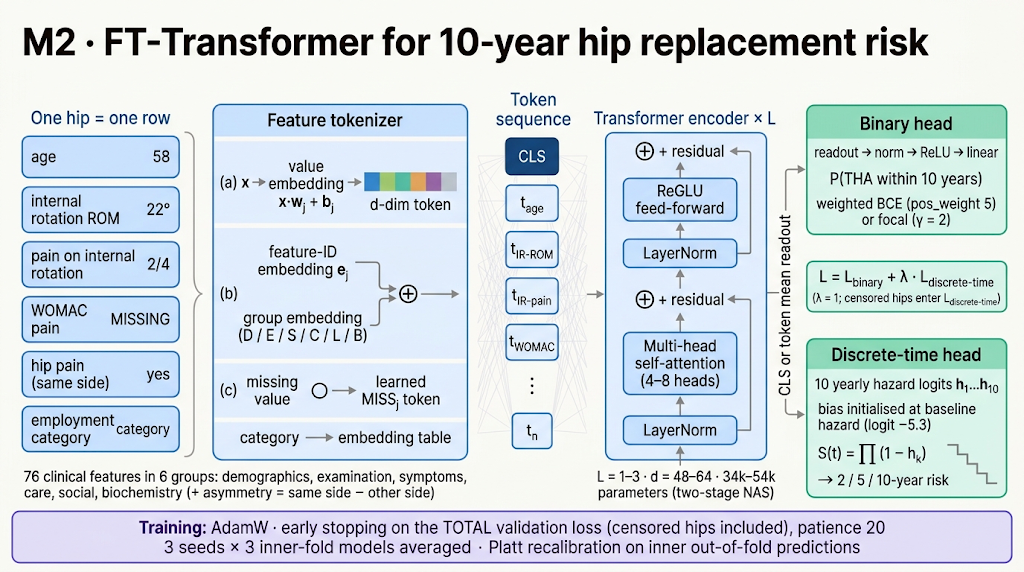
\includegraphics[width=\linewidth]{fig6_ftt.png}
  \caption{\textbf{M2 FT-Transformer.} Each hip is one row; every feature becomes a token (value embedding + feature-ID
  + group embedding; a learned [MISS]$_j$ token replaces missing values). Pre-norm Transformer blocks with residual
  connections feed a binary head and a discrete-time head with ten yearly hazards. The two are trained jointly
  ($\lambda=1$), and censored hips contribute through the discrete-time term.}
  \label{fig:ftt}
\end{figure}

\paragraph{M2: FT-Transformer and its stabilisation.}
M2~\cite{gorishniy2021fttransformer} stacks $L$ pre-norm blocks (multi-head self-attention, then a ReGLU feed-forward
layer), each wrapped in a residual connection. The loss is $\mathcal L=\mathcal L_{\text{bin}}+\lambda\mathcal
L_{\text{DT}}$. Here $\mathcal L_{\text{bin}}$ is weighted BCE (pos\_weight 5) or focal loss on hips with known status,
and $\mathcal L_{\text{DT}}$ is the discrete-time likelihood over all hips at risk. The first version had two faults. The
hazard bias started at 0, so the discrete-time head never trained, and early stopping on about 25 noisy validation
events made repeats unstable. The final recipe initialises the bias at the baseline hazard logit ($-5.3$), stops on the
total loss including censored hips, and averages three seeds. LayerNorm was compared with BatchNorm.

\paragraph{M3: image head.}
M3 uses an ImageNet DenseNet-121~\cite{huang2017densenet}, frozen, up to dense block 3. This yields a
$1024\times14\times14$ map in which one cell spans about a third of a head radius. The trainable head
(Fig.~\ref{fig:image-branch}; about 0.21\,M parameters) has four parts:
\begin{enumerate}[leftmargin=*,itemsep=0pt,topsep=2pt]
  \item a $1\times1$ convolution to 64 channels with BatchNorm;
  \item two residual blocks~\cite{he2016resnet};
  \item attention pooling~\cite{ilse2018attention} concatenated with global average pooling;
  \item one THA logit plus 11 auxiliary regressions onto the standardised OARSI items~\cite{altman2007oarsi}.
\end{enumerate}
The loss is $\mathrm{BCE}_{w=5}+\frac{1}{\sum_k m_k}\sum_k m_k(\hat r_k-\tilde r_k)^2$ over the available items $m_k$.
Readings are targets only, never inputs.

\paragraph{Training and cross-fitting of the image logit.}
The head trains for 30 fixed epochs (AdamW, 3-epoch warm-up, cosine decay, $\pm1$-cell shifts, Dropout2d 0.1). An inner
fold holds only about 25 events, too few for early stopping. Auxiliary targets are standardised within the training
fold. Within each outer training set the head is trained three times, each time without one inner fold, and scores the
hips of the fold it did not see. These out-of-fold logits are the image feature of the training hips. Test hips are
scored by a fourth head trained on the whole outer training set. M0 then refits with the logit as one extra feature
(stacking~\cite{wolpert1992stacked}).

\paragraph{}
Comparators were frozen PCA, a linear head, no auxiliary targets, AdaBN, SimCLR features, and [I]-token or FiLM fusion
of the frozen embedding into M2 (M4). Two follow-up runs were added. One fed the cross-fitted pixel logit as the [I]
token, with the same folds, architectures and single-seed recipe as the matching M2 run. The other (repeat 0)
restricted attention and average pooling to a disc of 1.6 head radii around the crop centre.

\begin{figure}[!tbp]
  \centering
  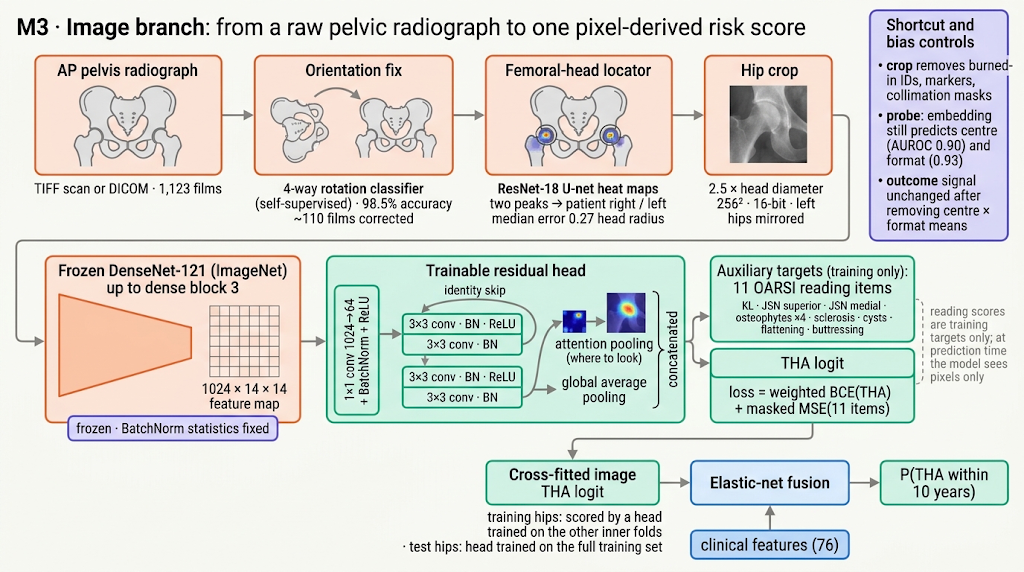
\includegraphics[width=\linewidth]{fig7_image_branch.png}
  \caption{\textbf{M3 image branch.} Raw film $\to$ orientation fix $\to$ femoral-head locator $\to$ hip crop $\to$
  frozen DenseNet-121 (block 3) $\to$ trainable residual head with attention pooling, supervised by the THA label and 11
  OARSI items (training only). The cross-fitted THA logit is the single image feature passed to the clinical elastic net.}
  \label{fig:image-branch}
\end{figure}

\paragraph{Hyper-parameter search and architecture search.}
Non-neural models were tuned by random search (40 configurations for M0, 60 for M1, 4 for M1b). Each outer fold selects
by Platt-recalibrated pooled inner log-loss, because inner AUPRC is unstable with about 25 events. M2 used a two-stage
search. Stage 1 scored 48 pre-sampled architectures (3.7k--56k parameters) on the inner folds of one outer split and kept
the best three. Stage 2 crossed them with lr $\{3\cdot10^{-4},10^{-3}\}$ and weight decay $\{10^{-5},10^{-4}\}$ inside
all 25 outer folds (Fig.~\ref{fig:hpo}; Table~\ref{tab:hparams}). The image head was not tuned.

\begin{figure}[!tbp]
  \centering
  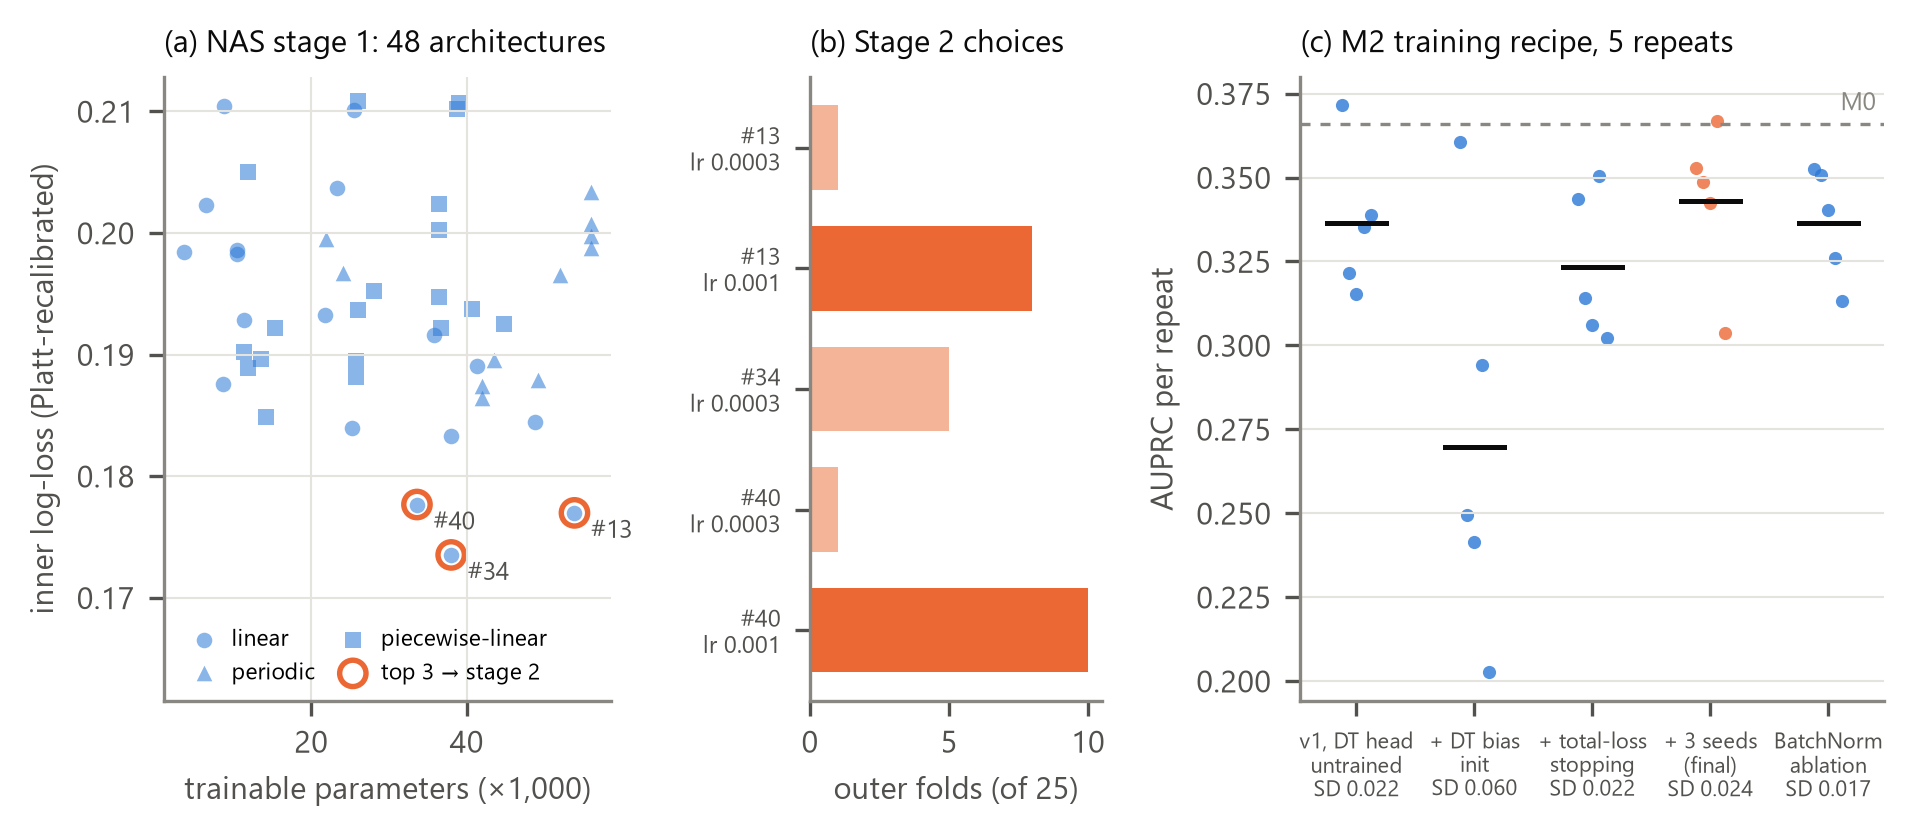
\includegraphics[width=\linewidth]{fig8_hpo_nas.png}
  \caption{\textbf{Hyper-parameter and architecture search.} (a) Stage-1 NAS: 48 FT-Transformer architectures, inner
  log-loss against size; the three best (circled) go to stage 2. (b) Configurations chosen across the 25 outer folds.
  (c) AUPRC of each repeat for successive M2 training recipes (bar = mean). The bias initialisation alone made the model
  unstable (SD 0.060), and early stopping on the total loss plus seed averaging restored stability (SD 0.024). The
  dashed line is M0.}
  \label{fig:hpo}
\end{figure}

% Table 2: final hyper-parameters. Sources: hpo/*.csv, oof/*_selection.csv, nas_stage1_DESCLB.csv, 08_imghead.py, lib_ftt.py
\begin{table}[!tbp]
  \centering
  \caption{\textbf{Search spaces and selected hyper-parameters.} ``Selected'' gives the configuration chosen most often
  across the 25 outer folds (count in brackets). M2's stage-2 choice varies by fold, so all three architectures are
  listed. The image head used fixed settings, chosen before training and not tuned per fold.}
  \label{tab:hparams}
  \small
  \setlength{\tabcolsep}{4pt}
  \begin{tabular}{@{}p{0.13\linewidth}p{0.40\linewidth}p{0.42\linewidth}@{}}
    \toprule
    Model & Search space & Selected / fixed \\
    \midrule
    M0 elastic net & 40 configs: $C\in[1.5\cdot10^{-3},9.6]$ (log), $\ell_1$ ratio $\{0,.1,.3,.5,.7,.9,1\}$, class
      weight \{none, balanced\}; SAGA & $C=0.012$, $\ell_1$ ratio 0.1, unweighted (10/25); next $C=0.082$, $\ell_1$ 0.3
      (6/25). The fusion model reuses this grid \\
    M1 LightGBM & 60 configs: leaves 4--31, depth 2--6, lr 0.01--0.10, min child 10--80, $\lambda_2$ 0.015--30,
      scale\_pos\_weight 1--20; early stop 100 rounds & leaves 31, depth 2, lr 0.042, min child 80, subsample 0.89,
      colsample 0.84, $\lambda_2$ 13.3, $\lambda_1$ 2.4, unweighted (5/25); median 232 trees \\
    M1b EBM & interactions \{0, 5\} $\times$ lr \{0.005, 0.02\}; 64 bins, min leaf 10, 8 outer bags & no interactions,
      lr 0.005 (16/25) \\
    M2 FT-Transformer & stage 1: 48 of $d\in\{16..64\}$, $L\in\{1,2,3\}$, heads \{2,4,8\}, FFN $\times$\{1, 4/3, 2\},
      dropouts 0--0.3, tokeniser \{linear, periodic, PLE\}, readout \{[CLS], mean\}, group emb.\ \{no, yes\}, loss
      \{wBCE, focal $\gamma$=1, 2\}; stage 2: top-3 $\times$ lr $\{3\!\cdot\!10^{-4},10^{-3}\}$ $\times$ wd
      $\{10^{-5},10^{-4}\}$ & \#40: $d$=64, $L$=1, 8 heads, [CLS], wBCE, 33.6k params (11/25); \#13: $d$=48, $L$=3, 4
      heads, mean, wBCE, 53.9k (9/25); \#34: $d$=48, $L$=2, 4 heads, mean, focal $\gamma$=2, 38.0k (5/25). All: linear
      tokeniser, group embedding, $\lambda$=1, pos\_weight 5, DT bias $-5.3$, AdamW, $\le$200 epochs, early stop on total
      loss (patience 20), 3 seeds $\times$ 3 inner folds \\
    M3 image head & fixed & frozen DenseNet-121 to block 3; 64 ch.; 2 residual blocks; attention + GAP; dropout 0.3,
      Dropout2d 0.1; AdamW lr $10^{-3}$, wd $10^{-3}$, batch 64, 30 epochs, 3-epoch warm-up + cosine; $\lambda_{\text{aux}}$=1,
      pos\_weight 5; 0.21\,M trainable params \\
    \bottomrule
  \end{tabular}
\end{table}


\paragraph{Interpretability.}
We applied three model-specific readouts on the repeat-0 outer test hips. For M2, we recorded the self-attention each
feature token receives, averaged over heads, blocks and the three inner-fold models. We report this as an
attention-allocation summary, not as an attribution. For M1, we computed exact TreeSHAP values~\cite{lundberg2017shap}.
For M3, we inspected attention-pooling maps of true positives, false positives and missed THAs. We also probed the head's
penultimate features against the 11 OARSI items (Spearman $\rho$, 5-fold) and compared them with frozen embeddings.

\paragraph{Auxiliary analyses.}
Six further analyses were run:
\begin{enumerate}[leftmargin=*,itemsep=0pt,topsep=2pt]
  \item feature-group increments and leave-one-group-out ablation;
  \item a temporal leakage audit: admissibility of each input at $t_0$, AUROC by time-to-THA window, and lag-2/3
        analyses that drop early events;
  \item shortcut probes~\cite{geirhos2020shortcut} for centre and format, before and after removing centre$\times$format
        means;
  \item pseudo-external transport~\cite{steyerberg2016validation} across ten pseudo-centres (recovered from DICOM device
        serials) and across format, pain, prior-care, sex and education splits, with participant-disjoint sources and
        source-only recalibration;
  \item forgetting monitors for SimCLR continued pretraining~\cite{chen2020simclr}: L2-SP~\cite{li2018l2sp}, a linear
        probe and CKA;
  \item calibration and decision curves~\cite{vickers2006dca}.
\end{enumerate}

% =============================================================================================
% 3 Results. Descriptive only; each paragraph <= 100 words. Orange = repeat-0 only / pending.
% Sources: results/results_all.csv, deltas.csv, temporal_*.csv, expB_*.csv, interp_*.csv (2026-10-24)
% =============================================================================================
\section{Results}
\label{sec:results}

\paragraph{Main model.}
A random model's AUPRC equals the event rate (5.5\%), so we report AUPRC with its lift (AUPRC $\div$ event rate). All
numbers are internal nested-CV estimates. The clinical elastic net reached AUPRC 0.366 (95\% CI 0.281--0.487; lift 6.7)
and AUROC 0.807 (0.771--0.868). Frozen DenseNet PCA-32 embeddings added little (AUPRC 0.386; $\Delta$ $+0.020$, $-0.049$
to $0.076$). The cross-fitted pixel logit raised AUPRC to 0.552 (0.472--0.685; lift 10.1) and AUROC to 0.892
(0.861--0.936): $\Delta$AUPRC $+0.203$ (0.121--0.287), $\Delta$AUROC $+0.078$ (0.042--0.121). LightGBM, EBM and the
FT-Transformer did not exceed M0 (all $\Delta$ CIs cross zero; Fig.~\ref{fig:models}).

\paragraph{Threshold metrics.}
At the 10\% risk threshold of the decision curve, the fusion model flagged 8.9\% of hips. It found 62\% of
replacements with precision 0.38 and MCC 0.45, against 54\%, 0.21 and 0.27 for M0 (Table~\ref{tab:threshold}). At
a fixed workload, the top 10\% of hips, sensitivity rose from 0.47 to 0.65. The three tabular comparators and the
FT-Transformer were within 0.03 MCC of M0. The image head alone reached MCC 0.44, close to the fusion model.

\begin{table}[!tbp]
  \centering
  \caption{\textbf{Threshold metrics at two operating points.} Left: calibrated risk $\ge$10\%, the threshold of the
  decision curve (the share of hips flagged depends on calibration). Right: the 10\% of hips with the highest risk (a
  fixed workload of about 170 hips, independent of calibration). Sensitivity, precision (positive predictive value) and
  Matthews correlation coefficient (MCC) are computed per repeat on pooled out-of-fold predictions and averaged over five
  repeats; the event rate is 5.5\%. The image head is calibrated on its cross-fitted inner predictions.}
  \label{tab:threshold}
  \small
  \setlength{\tabcolsep}{4pt}
  \begin{tabular}{@{}lccccccc@{}}
    \toprule
    & \multicolumn{4}{c}{Risk $\ge$ 10\%} & \multicolumn{3}{c}{Top 10\% of hips} \\
    \cmidrule(lr){2-5}\cmidrule(l){6-8}
    Model & Flagged & Sens. & Prec. & MCC & Sens. & Prec. & MCC \\
    \midrule
    M0 elastic net (clinical) & 14\% & 0.54 & 0.20 & 0.27 & 0.47 & 0.26 & 0.30 \\
    M1 LightGBM & 14\% & 0.54 & 0.21 & 0.28 & 0.48 & 0.26 & 0.30 \\
    M1b EBM & 13\% & 0.52 & 0.21 & 0.27 & 0.46 & 0.25 & 0.28 \\
    M2 FT-Transformer & 11\% & 0.48 & 0.23 & 0.28 & 0.46 & 0.25 & 0.29 \\
    M3 image head (pixels only) & 7\% & 0.54 & 0.41 & 0.44 & 0.61 & 0.34 & 0.41 \\
    \textbf{M0 + pixel logit (final)} & \textbf{9\%} & \textbf{0.62} & \textbf{0.38} & \textbf{0.45} & \textbf{0.65} & \textbf{0.35} & \textbf{0.44} \\
    \bottomrule
  \end{tabular}
\end{table}


\begin{figure}[!tbp]
  \centering
  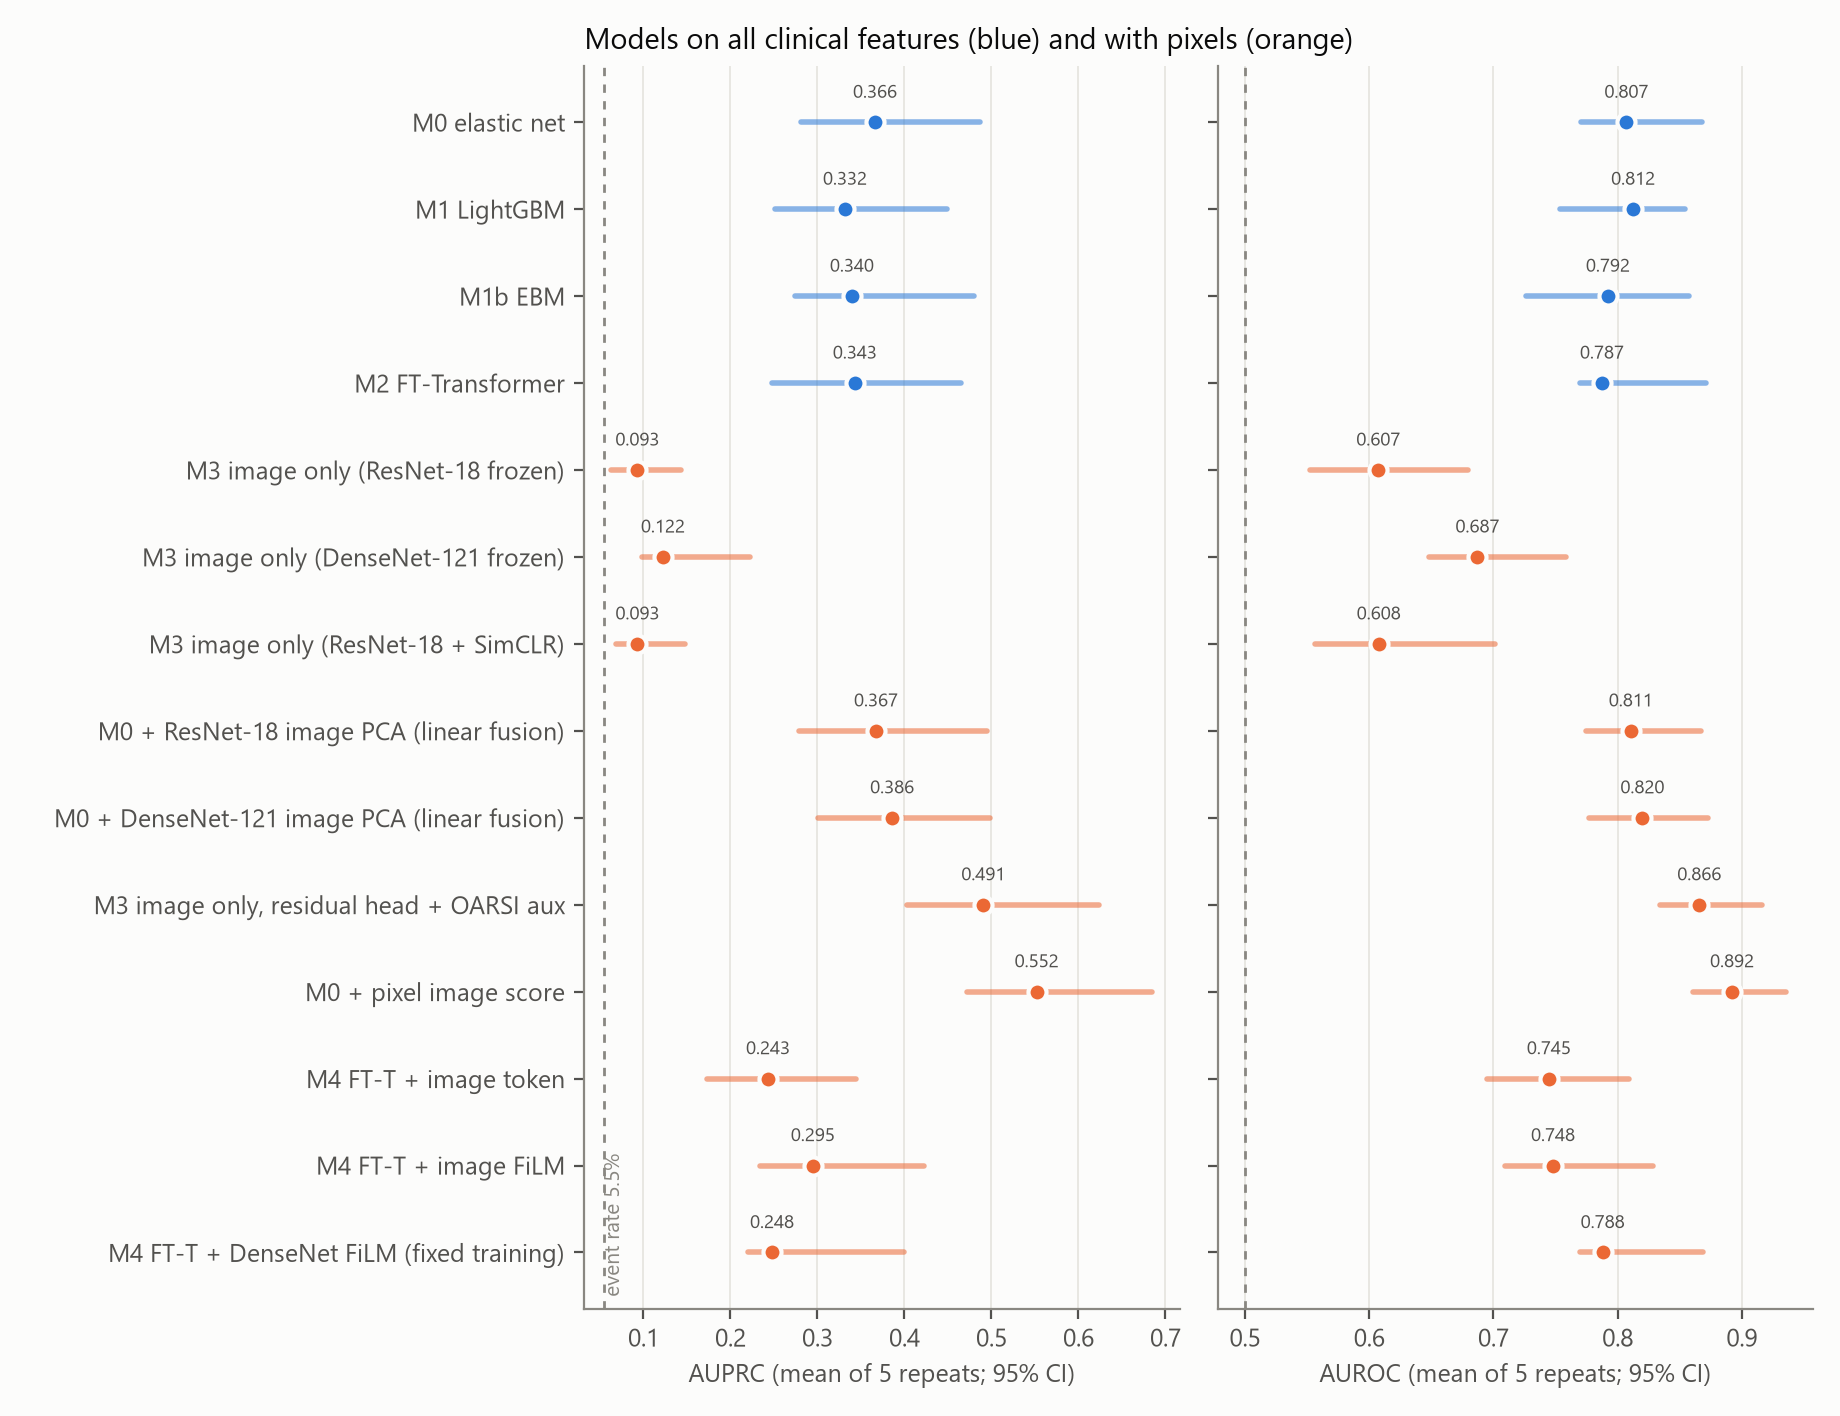
\includegraphics[width=\linewidth]{res_models_DESCLB.png}
  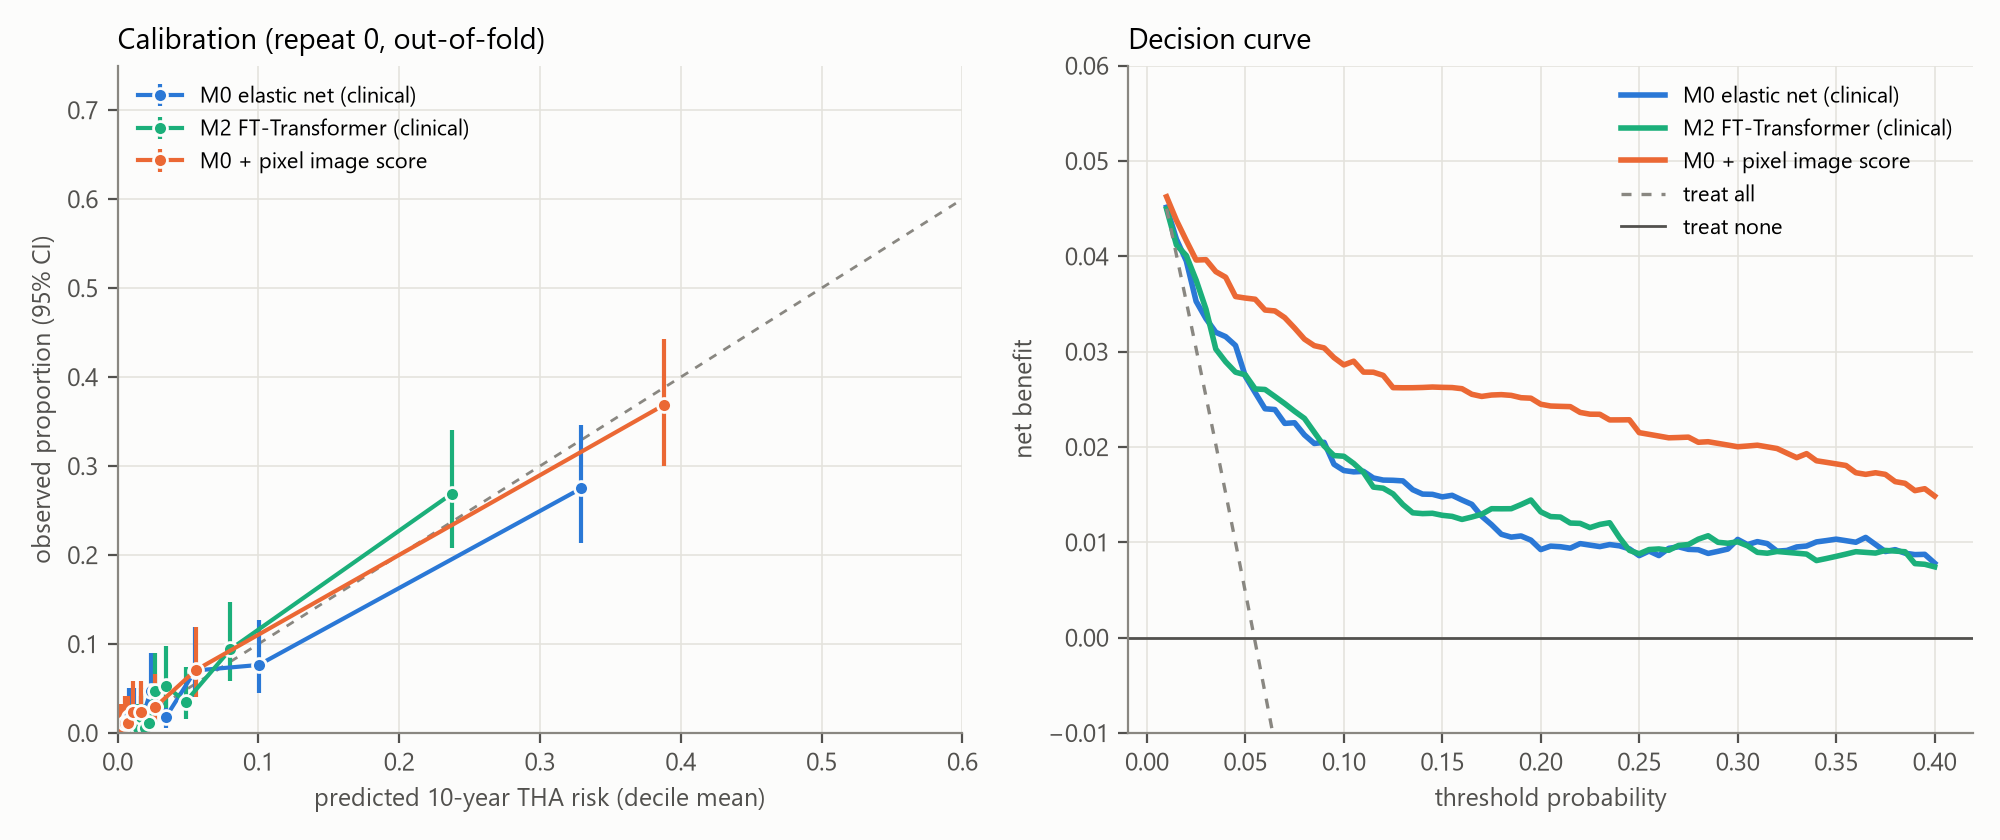
\includegraphics[width=\linewidth]{res_calibration_dca.png}
  \caption{\textbf{Model comparison, calibration and clinical utility.} Top: AUPRC and AUROC of all models on the full
  clinical set (blue) and with image information (orange); the dashed line is the event rate. Bottom: decile calibration
  and decision curves (repeat-0 out-of-fold predictions after Platt recalibration).}
  \label{fig:models}
\end{figure}

\paragraph{}
The FT-Transformer matched M0 in discrimination ($\Delta$AUPRC $-0.030$, $-0.082$ to $0.026$; AUROC 0.787) and had the
best calibration slope (1.04, against 0.84 for M0). Its discrete-time head gave usable 2- and 5-year rankings (AUROC 0.90
and 0.85). The training fixes changed stability more than level: the per-repeat SD of AUPRC fell from 0.060 to 0.024
(Fig.~\ref{fig:hpo}c). BatchNorm in place of LayerNorm gave AUPRC 0.337 (SD 0.017), so it was not adopted. The fusion
model's calibration slope was 0.79. At a 10\% decision threshold its net benefit was 0.029, against 0.018 for M0
(Fig.~\ref{fig:models}).

\paragraph{Image model.}
On pixels alone, frozen pooled features reached AUPRC 0.122 (0.098--0.222; AUROC 0.687), and a linear head on them
0.228 (AUROC 0.769). The residual head with auxiliary targets reached 0.491 (0.403--0.624; lift 9.0) and AUROC 0.866
(0.834--0.917), $+0.362$ (0.254--0.464) over
the frozen model. Most of the gain came from the spatial residual stage (linear $\to$ residual: $+0.268$,
0.154--0.362). Without auxiliary targets, discrimination was unchanged ($\Delta+0.011$, $-0.046$ to $0.072$), and the
calibration slope was 0.95 against 0.84. The supervised head recovered OARSI items better than frozen embeddings (KL
$\rho$ 0.31~$\to$~0.45; superior femoral osteophytes 0.24~$\to$~0.40).

\paragraph{}
In the attention maps (Fig.~\ref{fig:attention}), correctly ranked THA hips drew weight on the superolateral joint
space. False positives were mostly KL 1--2 hips with attention in the same place. Missed THA hips looked near-normal
(KL 0--1), and their attention fell on the medial pelvic wall. Quantified on repeat 0, THA hips ranked in the top 10\%
placed 69\% of their attention inside a disc of 1.6 head radii around the head centre. Missed THA hips placed 37\%
there, the same as unflagged hips (37\%) and close to uniform attention (31\%). Restricting attention and pooling to
that disc did not change performance (image only $\Delta$AUPRC $+0.004$, $-0.043$ to $0.056$; fusion $+0.003$,
$-0.026$ to $0.034$). The locator that defines the disc matched the annotated head circles with median Dice 0.82
(IoU 0.69; 279 heads, 3-fold CV).

\paragraph{} AdaBN lowered AUPRC ($-0.076$, $-0.130$ to $-0.027$).
SimCLR continued pretraining changed nothing ($+0.007$, $-0.031$ to $0.040$), even though the forgetting monitors stayed
healthy (probe log-loss 0.225~$\to$~0.213; CKA 0.59). Fusing the frozen embedding as an FT-Transformer token lowered
AUPRC by 0.132 relative to M0. With the cross-fitted pixel logit as the token, the FT-Transformer reached 0.471 (AUROC
0.848), still below the elastic-net fusion ($-0.095$, $-0.150$ to $-0.043$).

\begin{figure}[!tbp]
  \centering
  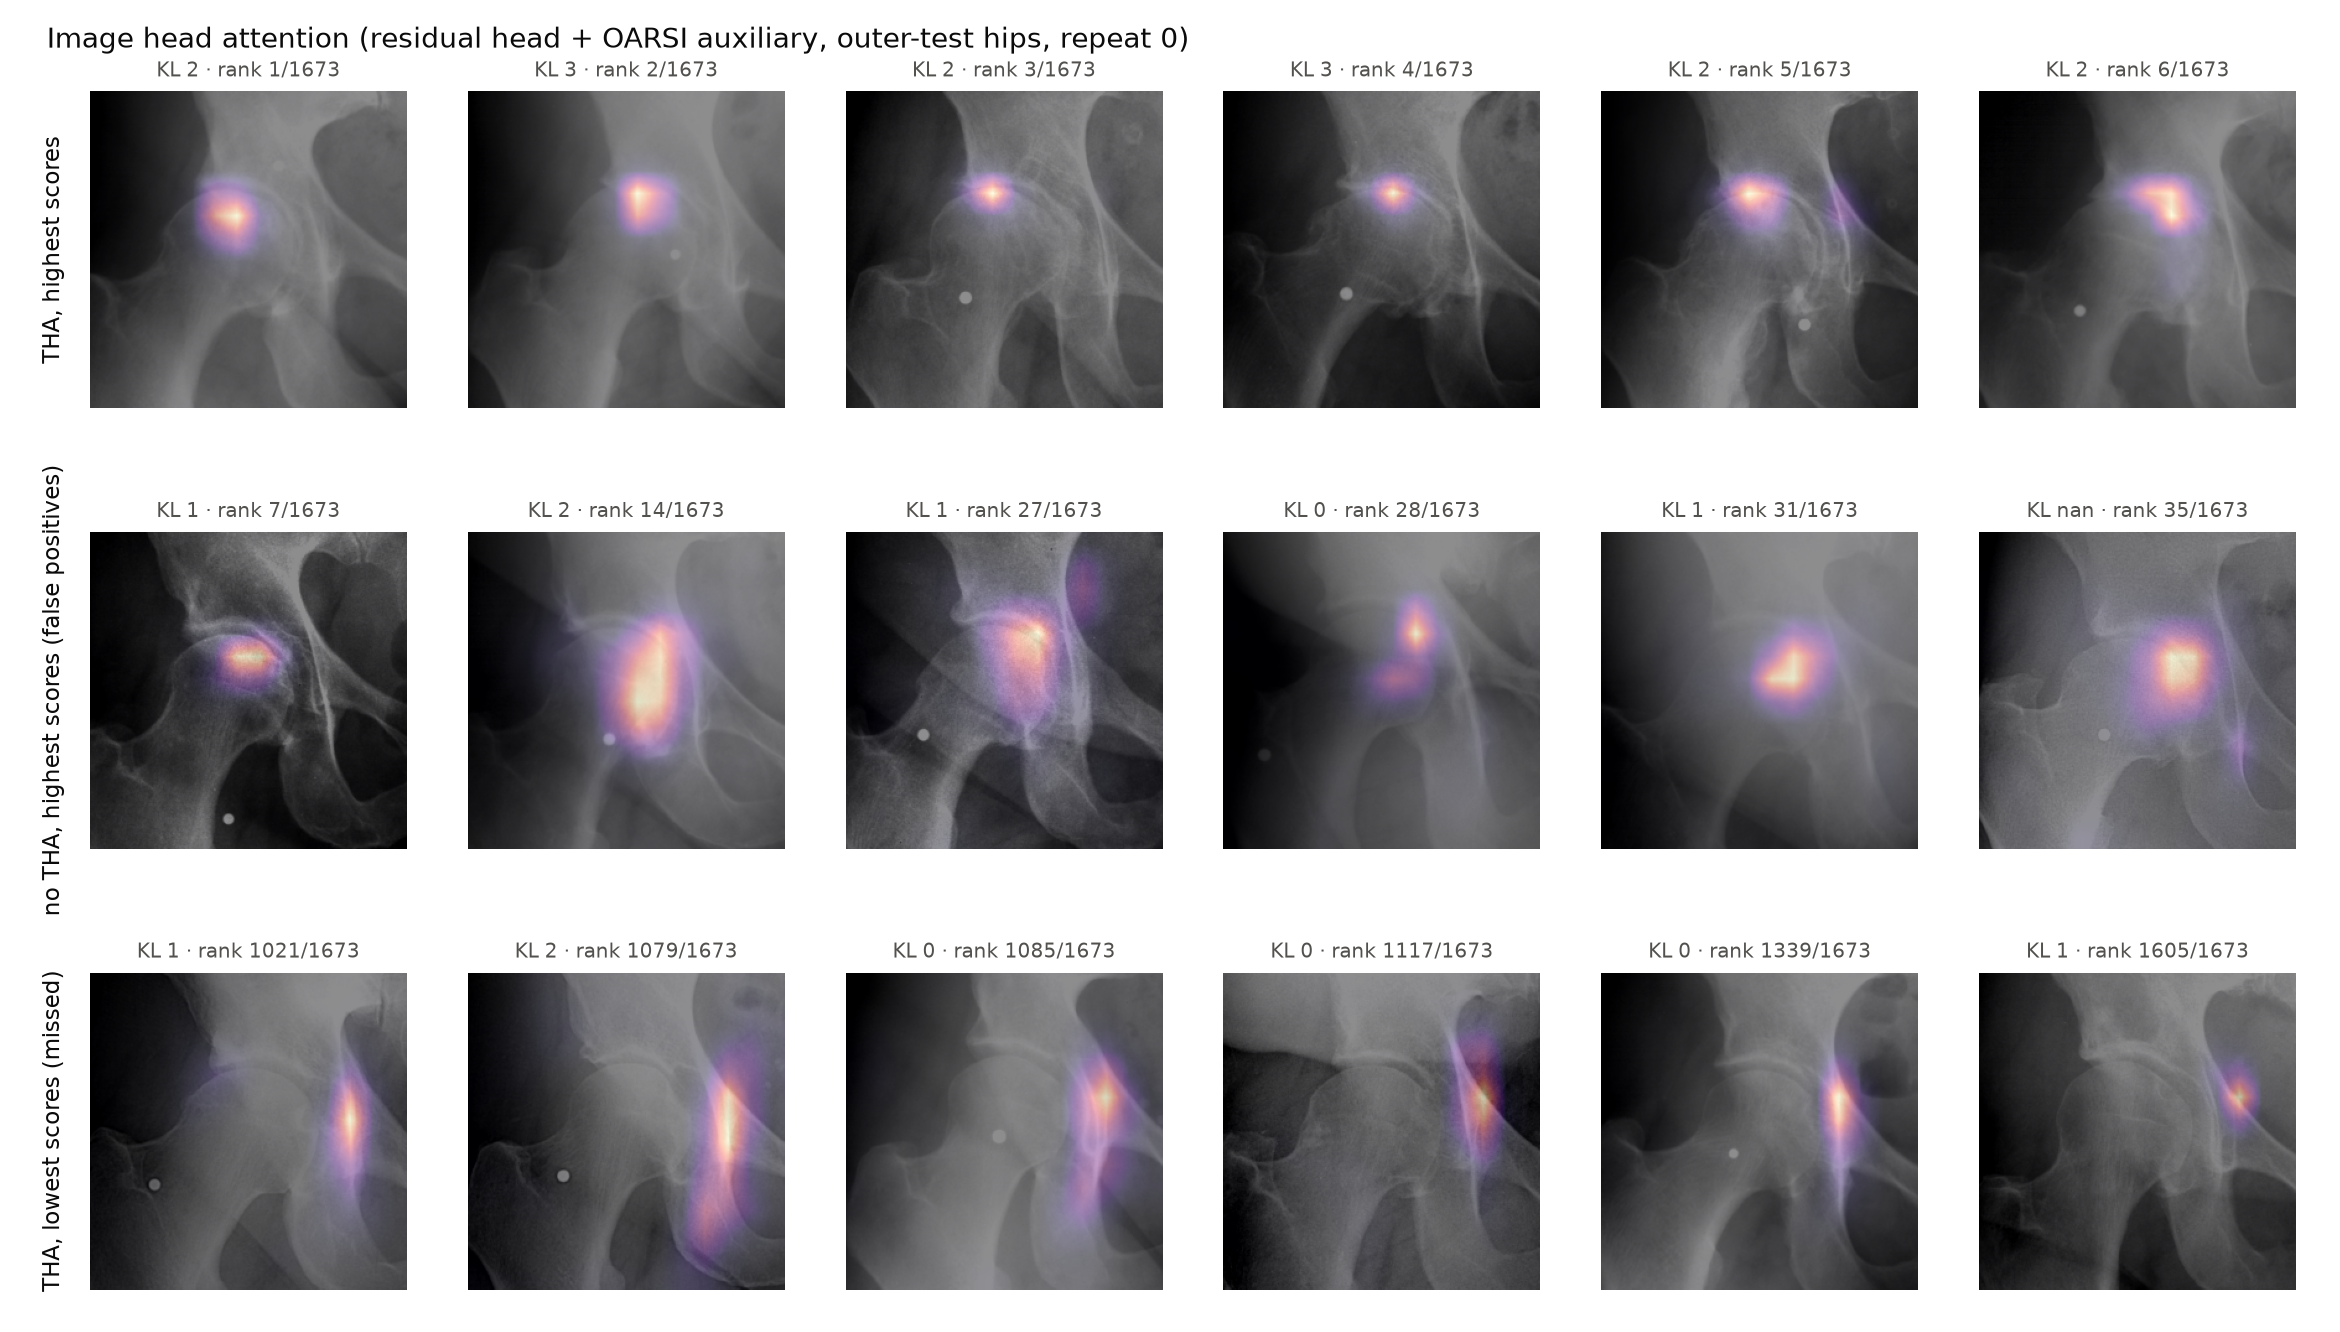
\includegraphics[width=\linewidth]{res_img_attention.png}
  \caption{\textbf{Attention pooling of the image head} on test hips: correctly ranked THA hips, false positives and
  missed THA hips (one outer fold of repeat~0). Weight concentrates on the superolateral joint space in THA hips and
  in KL 1--2 false positives. In missed cases, which look near-normal, it falls on the medial pelvic wall.}
  \label{fig:attention}
\end{figure}

\subsection{Auxiliary analyses}
\label{sec:res-aux}

\paragraph{Interpretability and feature-group ablation.}
The clinical signal lay in examination and symptoms: AUPRC rose from 0.092 (demographics, D) to 0.294 (+E) and 0.392
(+S), while care, social and biochemistry groups added nothing. Dropping E ($-0.081$, $-0.159$ to $-0.003$) or S
($-0.068$, $-0.136$ to $0.000$) hurt most (Fig.~\ref{fig:interp-tab}). FT-Transformer attention was nearly uniform, at most 1.16 times the uniform share. Its
ranking also did not reproduce: two identical reruns put examination tokens first and then demographic tokens first. We
therefore do not interpret it. TreeSHAP was deterministic and ranked comorbidity count, ipsilateral knee pain,
ipsilateral hip pain and internal-rotation ROM highest.

\begin{figure}[!tbp]
  \centering
  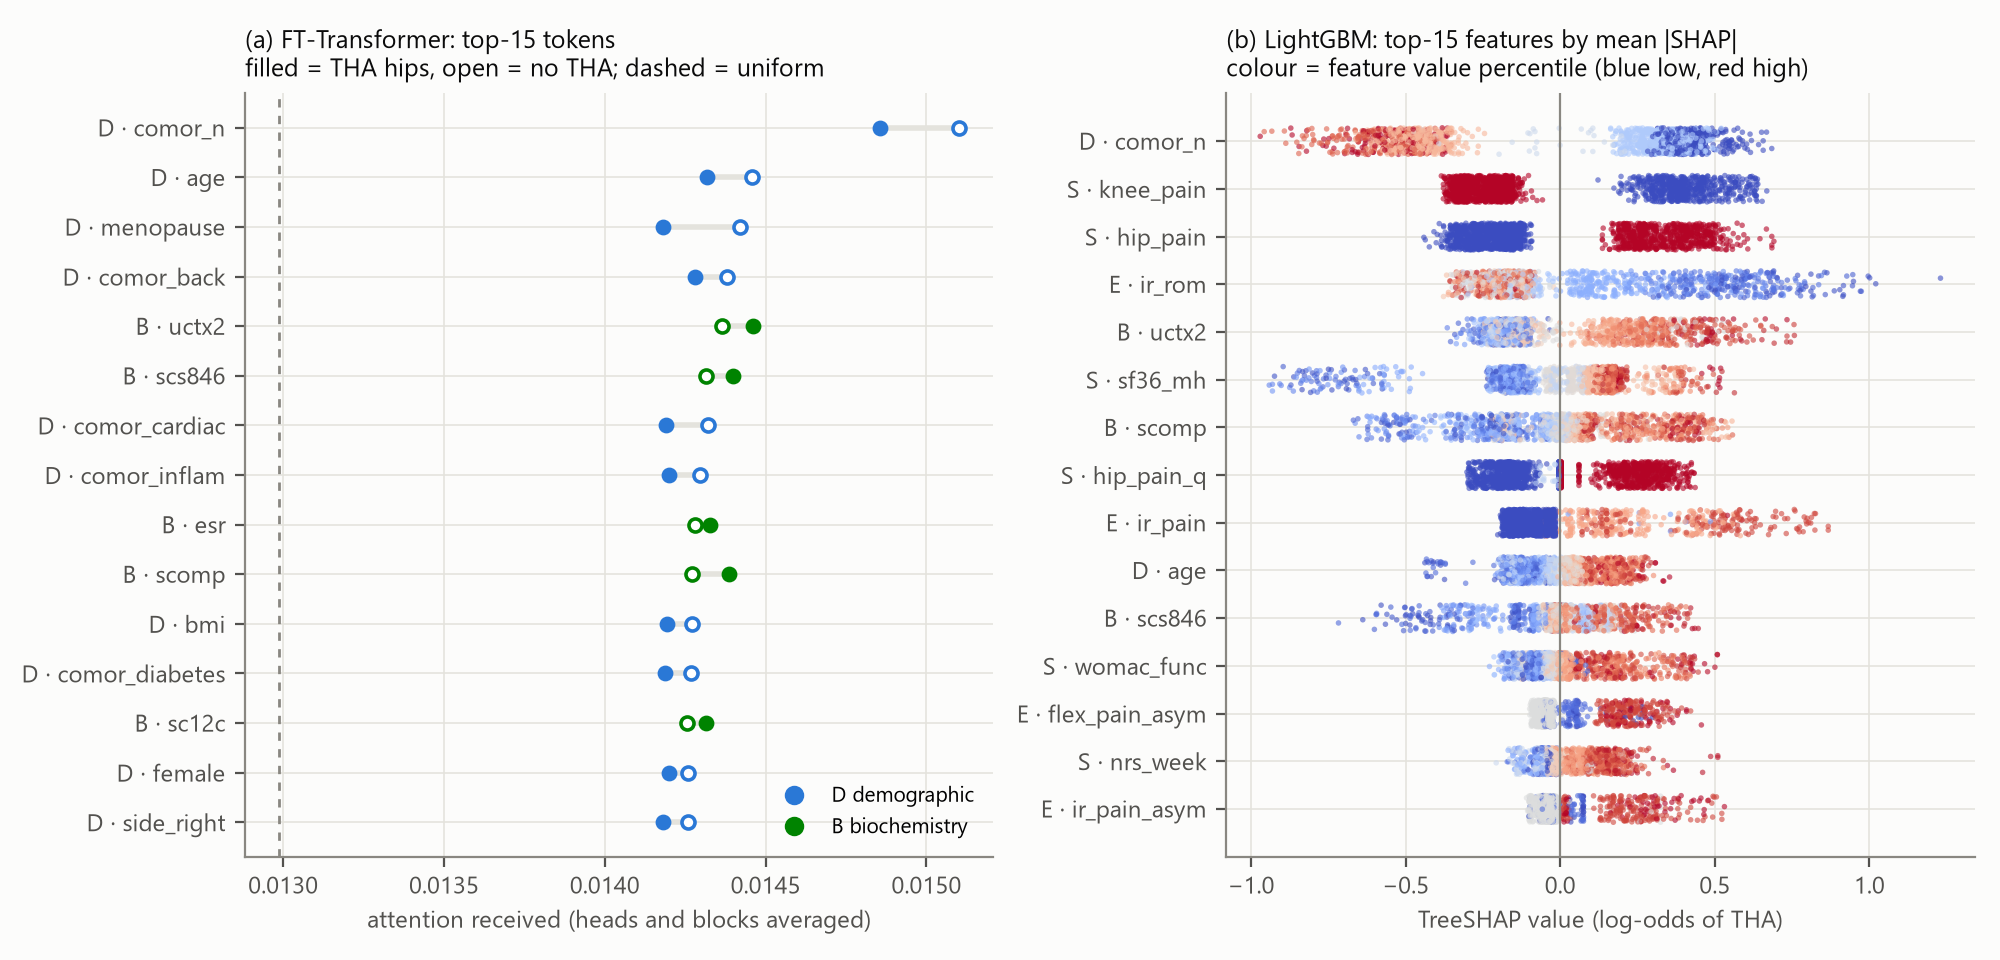
\includegraphics[width=\linewidth]{res_interp_tabular.png}
  \caption{\textbf{Tabular interpretability} (repeat-0 outer test hips). (a) FT-Transformer: attention received per
  token, for THA hips (filled) and the rest (open); the dashed line is uniform attention. All tokens lie within 16\% of
  uniform, and the ranking changed between identical reruns. (b) LightGBM TreeSHAP beeswarm; colour shows the
  feature-value percentile. Higher comorbidity counts and ipsilateral knee pain lower the predicted risk; knee pain marks
  ``bystander'' hips enrolled because of the knee. Hip pain and restricted internal rotation raise it.}
  \label{fig:interp-tab}
\end{figure}

\paragraph{Temporal leakage audit.}
Every input was fixed at $t_0$ (DICOM years 2003--2006; TIFF films in the baseline folder). The readings, the only
inadmissible input, enter no model. Discrimination fell with time to surgery for every model: AUROC was 0.90--0.98 for
THA in years 1--3 and 0.63--0.77 in years 8--10. Without THA in years 1--2, the fusion model reached AUROC 0.876 and
AUPRC 0.455, against 0.785 and 0.271 for M0 ($\Delta$AUPRC $+0.204$, 0.117--0.278). The head trained without readings
matched it ($+0.003$, $-0.062$ to $0.067$). The image score did not predict censoring (AUROC 0.52). One radiograph was
shared by two participants, affecting one THA hip.

\paragraph{Shortcut probes.}
Crop embeddings still identified the pseudo-centre (macro-AUROC 0.90) and the film format (0.93): grey-level handling,
resolution and post-processing remain in the pixels. Removing the centre$\times$format means within training folds
left the outcome probe unchanged (DenseNet 0.725 $\to$ 0.730). The follow-up-group probe dropped from 0.586 to 0.553.
Clinical tables also identified the centre (0.77) and the follow-up group (0.75), because the group was assigned by
symptom severity.

\paragraph{Pseudo-external transport.}
Under leave-one-centre-out validation, M0 kept its discrimination: pooled AUPRC 0.374 against 0.377 internally ($\Delta
-0.003$, $-0.049$ to $0.039$). Calibration did not transport: the intercept ranged from $-1.6$ to $+1.4$ across centres.
Painless hips were over-predicted (intercept $-1.47$; sensitivity 0.72, specificity 0.52 at the source threshold).
Discrimination dropped significantly only from the no-prior-care source to the prior-care target ($\Delta-0.128$,
$-0.220$ to $-0.028$). The image head transported across centres (AUROC 0.858 against 0.876) but lost
0.12--0.13 AUPRC across film formats (single fit, no CI; Appendix~\ref{app:transport}).

% =============================================================================================
% 4 Discussion + 5 Conclusion (v2, 2026-10-24 evening). Literature comparisons moved here from Results.
% =============================================================================================
\section{Discussion}
\label{sec:discussion}

\paragraph{The clinical model against prior work.}
Examination and symptoms carried the clinical signal: demographics alone reached AUPRC 0.09, adding the examination 0.29
and adding symptoms 0.39, whereas care, social and biomarker groups added nothing. The resulting elastic net (AUROC 0.81)
is well above the clinical GAM of the OAI study (0.68; Table~\ref{tab:main})~\cite{jang2023}. The difference is
plausibly the cohort rather than the learner. OAI is a knee cohort with little hip-specific examination, whereas CHECK
recorded a standardised hip examination and hip-specific questionnaires in people who presented early with hip
complaints. Restricted, painful internal rotation is part of the clinical definition of hip OA~\cite{altman1991acr}, and
in our data it carries more information than generic symptom scales. Deep tabular models did not beat the penalised
linear model at 93 events, as expected from the comparison literature~\cite{christodoulou2019}. The FT-Transformer's
contribution is a better calibration slope (1.04 against 0.84) and usable 2- and 5-year rankings.

\begin{table}[!tbp]
  \centering
  \caption{\textbf{Main-model performance against published multimodal models.} Our rows are internal estimates: means
  over five repeats of 5-fold nested CV, with 95\% CIs from a participant-clustered bootstrap of repeat 0. Lift = AUPRC
  $\div$ event rate. Literature values are from the abstracts and, where available, the full texts. \textsuperscript{\dag}Different endpoint
  (radiographic OA or KL progression); shown for scale only.}
  \label{tab:main}
  \small
  \setlength{\tabcolsep}{3.5pt}
  \resizebox{\linewidth}{!}{%
  \begin{tabular}{@{}llcccc@{}}
    \toprule
    Study / model & Cohort, endpoint & Event rate & AUPRC (95\% CI) & Lift & AUROC (95\% CI) \\
    \midrule
    Jang 2023, clinical GAM~\cite{jang2023} & OAI, THA 10 y & 2.4\% & 0.08 & 3.3 & 0.68 \\
    Jang 2023, clinical + DL measurements & OAI, THA 10 y & 2.4\% & 0.28 & 11.7 & 0.81 \\
    Musbahi 2026, DenseNet-201 + clinical~\cite{musbahi2026} & MOST, TKA & $\approx$10\% & 0.62 & 6.2 & 0.85 (ext.\ 0.79) \\
    Gielis 2020, clinical + Shape-Score~\cite{gielis2020}\textsuperscript{\dag} & CHECK, rHOA/THA 8 y & 17.7\% & -- & -- & 0.864 (0.833--0.895) \\
    van den Berg 2026, hybrid~\cite{vandenberg2026}\textsuperscript{\dag} & 7 cohorts, rHOA 4--8 y & 5.1\% & -- & -- & 0.81 (LOCO 0.64) \\
    Tiulpin 2019, CNN + clinical~\cite{tiulpin2019}\textsuperscript{\dag} & OAI$\to$MOST, knee KL & 38\% & 0.68 (0.66--0.70) & 1.8 & 0.79 (0.78--0.81) \\
    \midrule
    \textbf{M0} clinical elastic net & CHECK, THA 10 y & 5.5\% & 0.366 (0.281--0.487) & 6.7 & 0.807 (0.771--0.868) \\
    M0 + frozen DenseNet PCA-32 (v1) & CHECK, THA 10 y & 5.5\% & 0.386 (0.301--0.499) & 7.1 & 0.820 (0.777--0.873) \\
    \textbf{M0 + pixel logit (final)} & CHECK, THA 10 y & 5.5\% & \textbf{0.552} (0.472--0.685) & \textbf{10.1} & \textbf{0.892} (0.861--0.936) \\
    \bottomrule
  \end{tabular}}
\end{table}

\paragraph{Transport across centres.}
Discrimination transported across pseudo-centres: under leave-one-centre-out validation M0 kept its AUPRC (0.374 against
0.377 internally) and lost 0.02 AUROC, and the image head lost 0.02 AUROC. Published hip models fare worse under the
same design. A seven-cohort model fell from AUROC 0.81 to 0.64 under leave-one-cohort-out validation~\cite{vandenberg2026},
and a knee surgical model fell from 0.85 to 0.79 externally~\cite{musbahi2026}. Clinical-only knee models are known to
transport well~\cite{castagno2025}, and our result extends this to the hip with a standardised examination. The
comparison flatters us, however. Our pseudo-centres share country, era, protocol and readers, so the shift between them
is milder than between cohorts. Calibration did not transport (intercepts $-1.6$ to $+1.4$; painless hips
over-predicted), and image discrimination was sensitive to film format. Local recalibration is therefore a precondition
for use, as for most prediction models~\cite{steyerberg2016validation}.

\paragraph{The image numbers in a rare-event setting.}
At a 5.5\% event rate, an image-only AUROC of 0.87 and a fusion gain of $+0.20$ AUPRC (0.37 $\to$ 0.55) must be read on
the precision scale. The highest attainable lift is the inverse of the event rate: 18 here and 42 in OAI. Our fused lift
of 10.1 thus uses about half of the available range, and Jang's 11.7 about a quarter of its range. The image-only head
(lift 9.0) matches Jang's measurement model (9.2) at twice the event rate (Table~\ref{tab:image}). The more
important question is where the gain comes from. Radiographic severity is a core indication for THA: surgeons offer
replacement when symptoms persist \emph{and} the film shows advanced joint damage~\cite{gademan2016indication}. The
baseline film therefore carries part of the decision that defines the outcome, and the gain is concentrated in hips
replaced within 1--3 years (AUROC 0.90--0.98 for every model). In our reading, the improvement reflects what the image
contains rather than an advantage of attention as a mechanism. The architecture mattered only for extraction. The same
pixels gave AUPRC 0.12 through frozen pooled features and 0.49 through the spatial head.

\begin{table}[!tbp]
  \centering
  \caption{\textbf{Image-only performance.} Same conventions as Table~\ref{tab:main}.
  \textsuperscript{\dag}Different endpoint (shown for scale only).}
  \label{tab:image}
  \small
  \setlength{\tabcolsep}{3.5pt}
  \resizebox{\linewidth}{!}{%
  \begin{tabular}{@{}llcccc@{}}
    \toprule
    Study / model & Cohort, endpoint & Event rate & AUPRC (95\% CI) & Lift & AUROC (95\% CI) \\
    \midrule
    Agricola 2013, shape modes (apparent)~\cite{agricola2013} & CHECK, THA 5 y & 2.5\% & -- & -- & 0.81 \\
    Jang 2023, 26 DL measurements~\cite{jang2023} & OAI, THA 10 y & 2.4\% & 0.22 & 9.2 & 0.77 \\
    van den Berg 2026, DL features~\cite{vandenberg2026}\textsuperscript{\dag} & 7 cohorts, rHOA 4--8 y & 5.1\% & -- & -- & 0.81 \\
    Tiulpin 2019, CNN~\cite{tiulpin2019}\textsuperscript{\dag} & OAI$\to$MOST, knee KL & 38\% & 0.68 (0.66--0.70) & 1.8 & 0.79 (0.77--0.80) \\
    \midrule
    Frozen DenseNet-121, GAP + PCA-32 & CHECK, THA 10 y & 5.5\% & 0.122 (0.098--0.222) & 2.2 & 0.687 (0.649--0.758) \\
    Linear head on GAP features & CHECK, THA 10 y & 5.5\% & 0.228 (0.176--0.370) & 4.2 & 0.769 (0.723--0.829) \\
    \textbf{Residual head + OARSI targets} & CHECK, THA 10 y & 5.5\% & \textbf{0.491} (0.403--0.624) & \textbf{9.0} & \textbf{0.866} (0.834--0.917) \\
    \bottomrule
  \end{tabular}}
\end{table}

\paragraph{Why the image head works, and what it may be reading.}
Several observations support a genuine pixel signal. Most of the gain came from the spatial residual stage (linear
$\to$ residual: $+0.27$ AUPRC). Attention concentrated on the superolateral joint space, the typical site of early
narrowing in hip OA. The head recovered OARSI items better than frozen features did (KL $\rho$ 0.31 $\to$ 0.45). A head
trained without the reading targets fused equally well (AUPRC 0.527 against 0.552), and without THA in years 1--2 the
fusion gain remained $+0.20$. Other observations argue for caution. False positives were KL 1--2 hips with attention in
the same place. This suggests the head encodes radiographic stage, which is partly the surgeon's decision rule, rather
than biology that predicts progression. In missed hips the attention drifted away from the joint, but confining it to
the joint did not recover them. The drift is therefore a symptom of finding no signal, not the cause of the miss.
Crop embeddings still identified the centre and the format. Attention maps are descriptive, not attributions. With observational data we cannot separate these explanations causally.

\paragraph{Why token fusion failed.}
Fusing the image as one FT-Transformer token lowered AUPRC by 0.13 relative to M0. The likely cause is the input to
the token, not the transformer. M4 received the frozen embedding after global pooling and PCA to 32 dimensions. That
signal was weak on its own (AUPRC 0.12), because pooling discards the location of millimetre-scale joint-space changes.
The token's input LayerNorm then normalised each hip's 32-vector, which removes its magnitude. With about 60 events
per training fold, the attention layers had to learn a cross-modal interaction from a weak, noisy token. A follow-up
run supports this reading. Feeding the cross-fitted pixel logit as the token (with the LayerNorm bypassed) raised the
FT-Transformer from 0.323 to 0.471 AUPRC ($+0.147$, 0.038--0.250; AUROC 0.848, calibration slope 0.99). Its 10-year
discrete-time risk reached AUROC 0.83. It remained below the elastic-net fusion ($-0.095$, $-0.150$ to $-0.043$). The
transformer is therefore not useless, but at this sample size an extra layer of interactions costs more than it gains.

\paragraph{Clinical implications.}
The model gives a first-visit risk score from routine data and the raw film, without a radiologist's grading. Its
intended uses are setting the intensity of conservative care and the review interval, timing referral, and enriching
joint-preservation trials with high-risk hips. It adds little for hips already on a surgical pathway, where THA follows
within two years and any model performs well. Before use elsewhere it needs local recalibration, especially for hips
without pain.

\paragraph{Limitation 1: data scale against model capacity.}
Deep networks learn their representations from very large data sets: ImageNet has 1.2 million labelled images. We
have 1,705 hips with known outcome, and for a binary outcome the effective sample size is closer to the 93 events. On
the course's rule of thumb (Lecture 2, slide 107), our 1,968 films sit in the regime where fine-tuning works, but the
93 positives sit in the ``marginal'' range of high dozens to low hundreds. We therefore never trained a deep network
end to end. The image backbone was pretrained on ImageNet and frozen. Only a
0.21\,M-parameter head was trained on pixels, and the FT-Transformer had 34k--56k parameters. Even so, the
FT-Transformer did not beat a penalised linear model, its repeats were unstable until seeds were averaged, and the
fusion model's calibration slope of 0.79 shows residual overfitting. The event count, not the architecture, limits
what this study can show about deep models. It does not explain the AUPRC level, which is bounded by the 5.5\% event
rate, as discussed above.

\paragraph{Further limitations of the statistical design.}
Three further issues could not be resolved within this study. First, events per parameter: 93 events against 76
features plus missing indicators is about one event per candidate parameter, below current
guidance~\cite{riley2020samplesize}. Penalisation limits overfitting but does not remove it. Second, imputation: fold-wise MICE is a single imputation under a missing-at-random assumption, so it understates
uncertainty. It also excludes the outcome, which biases imputed predictors' effects towards zero~\cite{moons2006imputation,
vanbuuren2011mice}. Collinearity is a minor concern here. BayesianRidge shrinks correlated predictors, and correlated
predictors make imputation more accurate. Because only 2--5\% of values were imputed, the impact is small. Third,
censoring: excluding the 299 hips censored before year 10 conditions on follow-up, and death as a competing risk was
not recorded.

\paragraph{Limitations of the image supervision and the stacking.}
The OARSI targets may reduce generalisation. They encode the conventions of CHECK's readers and a paired reading with
later films~\cite{macri2022}, so the head may learn features that do not transfer to cohorts read differently. World
COACH faced the same issue: its best image features were optimised with follow-up grades~\cite{vandenberg2026}. Our
no-target head matched discrimination internally, but its transport was not tested externally. The cross-fitting
itself does not leak test labels. Each training hip's logit comes from a head that never saw that hip, test hips are
scored by a head trained only on training hips, and test labels are used only for evaluation. Two weaker effects
remain. Training logits come from heads fitted on two thirds of the data, so their scale differs slightly from the test
logits. During inner tuning, inner-validation labels have shaped other training hips' logits. Both effects can bias
the choice of hyper-parameters, but not the outer-fold estimate.

\paragraph{Limitations of late fusion.}
The final model fuses late: the image head is trained on pixels alone, and its logit enters the elastic net as one
feature. Because the logit is fitted jointly with the clinical features, its coefficient is already adjusted for
their linear correlation. Late fusion still has two costs. The head never sees the clinical context, so part of what
it learns duplicates the examination. And a single linear term cannot express interactions, for example a pixel
signal that matters more in painful hips. Joint fusion is the alternative. Here it lost at this sample size, both as a
frozen-embedding token and FiLM (M4) and as a pixel-logit token (AUPRC 0.471 against 0.552). Training the head on the
residual of the clinical model, or adding pre-specified interaction terms, are cheaper middle grounds for future work.

\paragraph{Limitations of the cohort.}
CHECK enrolled Dutch adults aged 45--65 with early complaints between 2002 and 2005. Of these, 79\% were women and 97\%
were white, and more than half had not seen any health professional for the complaint in the year before baseline.
Referral passes through general practitioners, and both the threshold for surgery and access to it are specific to
that health system and era. The model may therefore not hold for older patients, for populations with different hip
morphology or OA prevalence (for example, East Asian cohorts with more dysplasia-related OA), or where access to
surgery differs. Validation was internal only. The pseudo-centres were reconstructed from device serials, two of them
impurely. Label-free steps (orientation, locator, SimCLR, AdaBN) were fitted on all films.

\paragraph{Future work.}
The first priority is external validation, in OAI hip films and in the World COACH consortium. Both would test format
and population transport, and both would show whether local recalibration is enough. On the imaging side, end-to-end
fine-tuning with an L2-SP penalty would let the backbone adapt to radiographs without forgetting its pretraining.
Higher resolution ($28\times28$ maps or $512^2$ crops) would target cysts and head flattening, which the current map
resolves poorly. Explicit geometric measurements (lateral centre-edge angle, $\alpha$ angle, minimum joint-space width)
would make the pixel score interpretable, and a contralateral-hip reference could separate a person's anatomy from
disease. Format harmonisation should reduce the TIFF/DICOM gap. Finally, decision thresholds should be set with
clinicians through decision-curve analysis rather than chosen by us.

\section{Conclusion}
\label{sec:conclusion}
We asked whether a first-consultation hip can be scored for ten-year replacement risk from routine information alone. In
the CHECK study, a penalised logistic model on the standardised hip examination and symptoms already discriminates well
(AUROC 0.81), and deep tabular models do not improve on it at 93 events. Frozen ImageNet features of the baseline film
add nothing. A small residual head that keeps the spatial map of a frozen DenseNet, trained with OARSI items as
targets only, extracts a strong pixel signal. Fused as one cross-fitted logit, it raises AUPRC from 0.37 to 0.55 in
internal validation, and the gain survives the exclusion of early events. Much of this signal reflects radiographic
stage, which is itself a criterion for surgery. Discrimination transported across pseudo-centres, but calibration did
not. The model is therefore a candidate for external validation and local recalibration, not a finished tool.


\paragraph{Code and demo availability.} The code behind every number and figure in this report, the LaTeX source and
the LecTrace lecture are at \url{\repourl}. GitHub Actions deploys the lecture to GitHub Pages at \url{\demourl}; its
source is \texttt{lectrace/01\_seeing\_surgery\_coming.py}. Raw CHECK data are not redistributed; they can be obtained
from DANS (below).

\begin{ack}
The CHECK-cohort study is funded by the Dutch Arthritis Foundation. Involved are: Erasmus Medical Center Rotterdam;
Kennemer Gasthuis Haarlem; Leiden University Medical Center; Maastricht University Medical Center; Martini Hospital
Groningen/Allied Health Care Center for Rheumatology and Rehabilitation Groningen; Medical Spectrum Twente
Enschede/Ziekenhuisgroep Twente Almelo; Reade Center for Rehabilitation and Rheumatology; St.Maartens-kliniek Nijmegen;
University Medical Center Utrecht and Wilhelmina Hospital Assen.
Data: DANS, doi:10.17026/DANS-XEX-HZWW (CC BY 4.0).
\end{ack}

{\small
\bibliographystyle{unsrtnat}
\bibliography{refs}
}

\appendix
% =============================================================================================
% Appendix
% =============================================================================================
\section{Exploratory data analysis (supplementary figures)}
\label{app:eda}
\setcounter{figure}{0}
\renewcommand{\thefigure}{S\arabic{figure}}

\begin{figure}[!htbp]
  \centering
  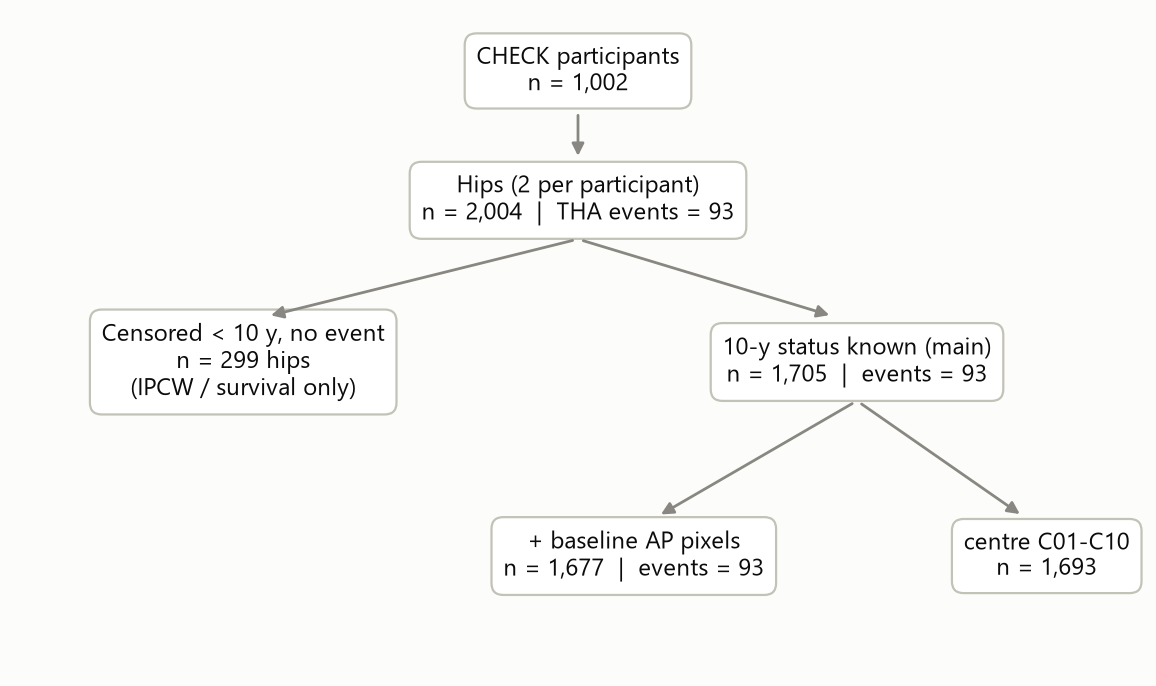
\includegraphics[width=0.78\linewidth]{figS1_flow.png}
  \caption{\textbf{Cohort flow.} 1,002 participants contribute 2,004 hips and 93 THAs. The 299 hips censored before
  year 10 without an event are excluded from the binary analysis and enter only the discrete-time head. Of the 1,705
  hips with known status, 1,677 have baseline AP pixels (every THA hip), and 1,693 belong to a recovered centre.}
  \label{fig:s-flow}
\end{figure}

\begin{figure}[!htbp]
  \centering
  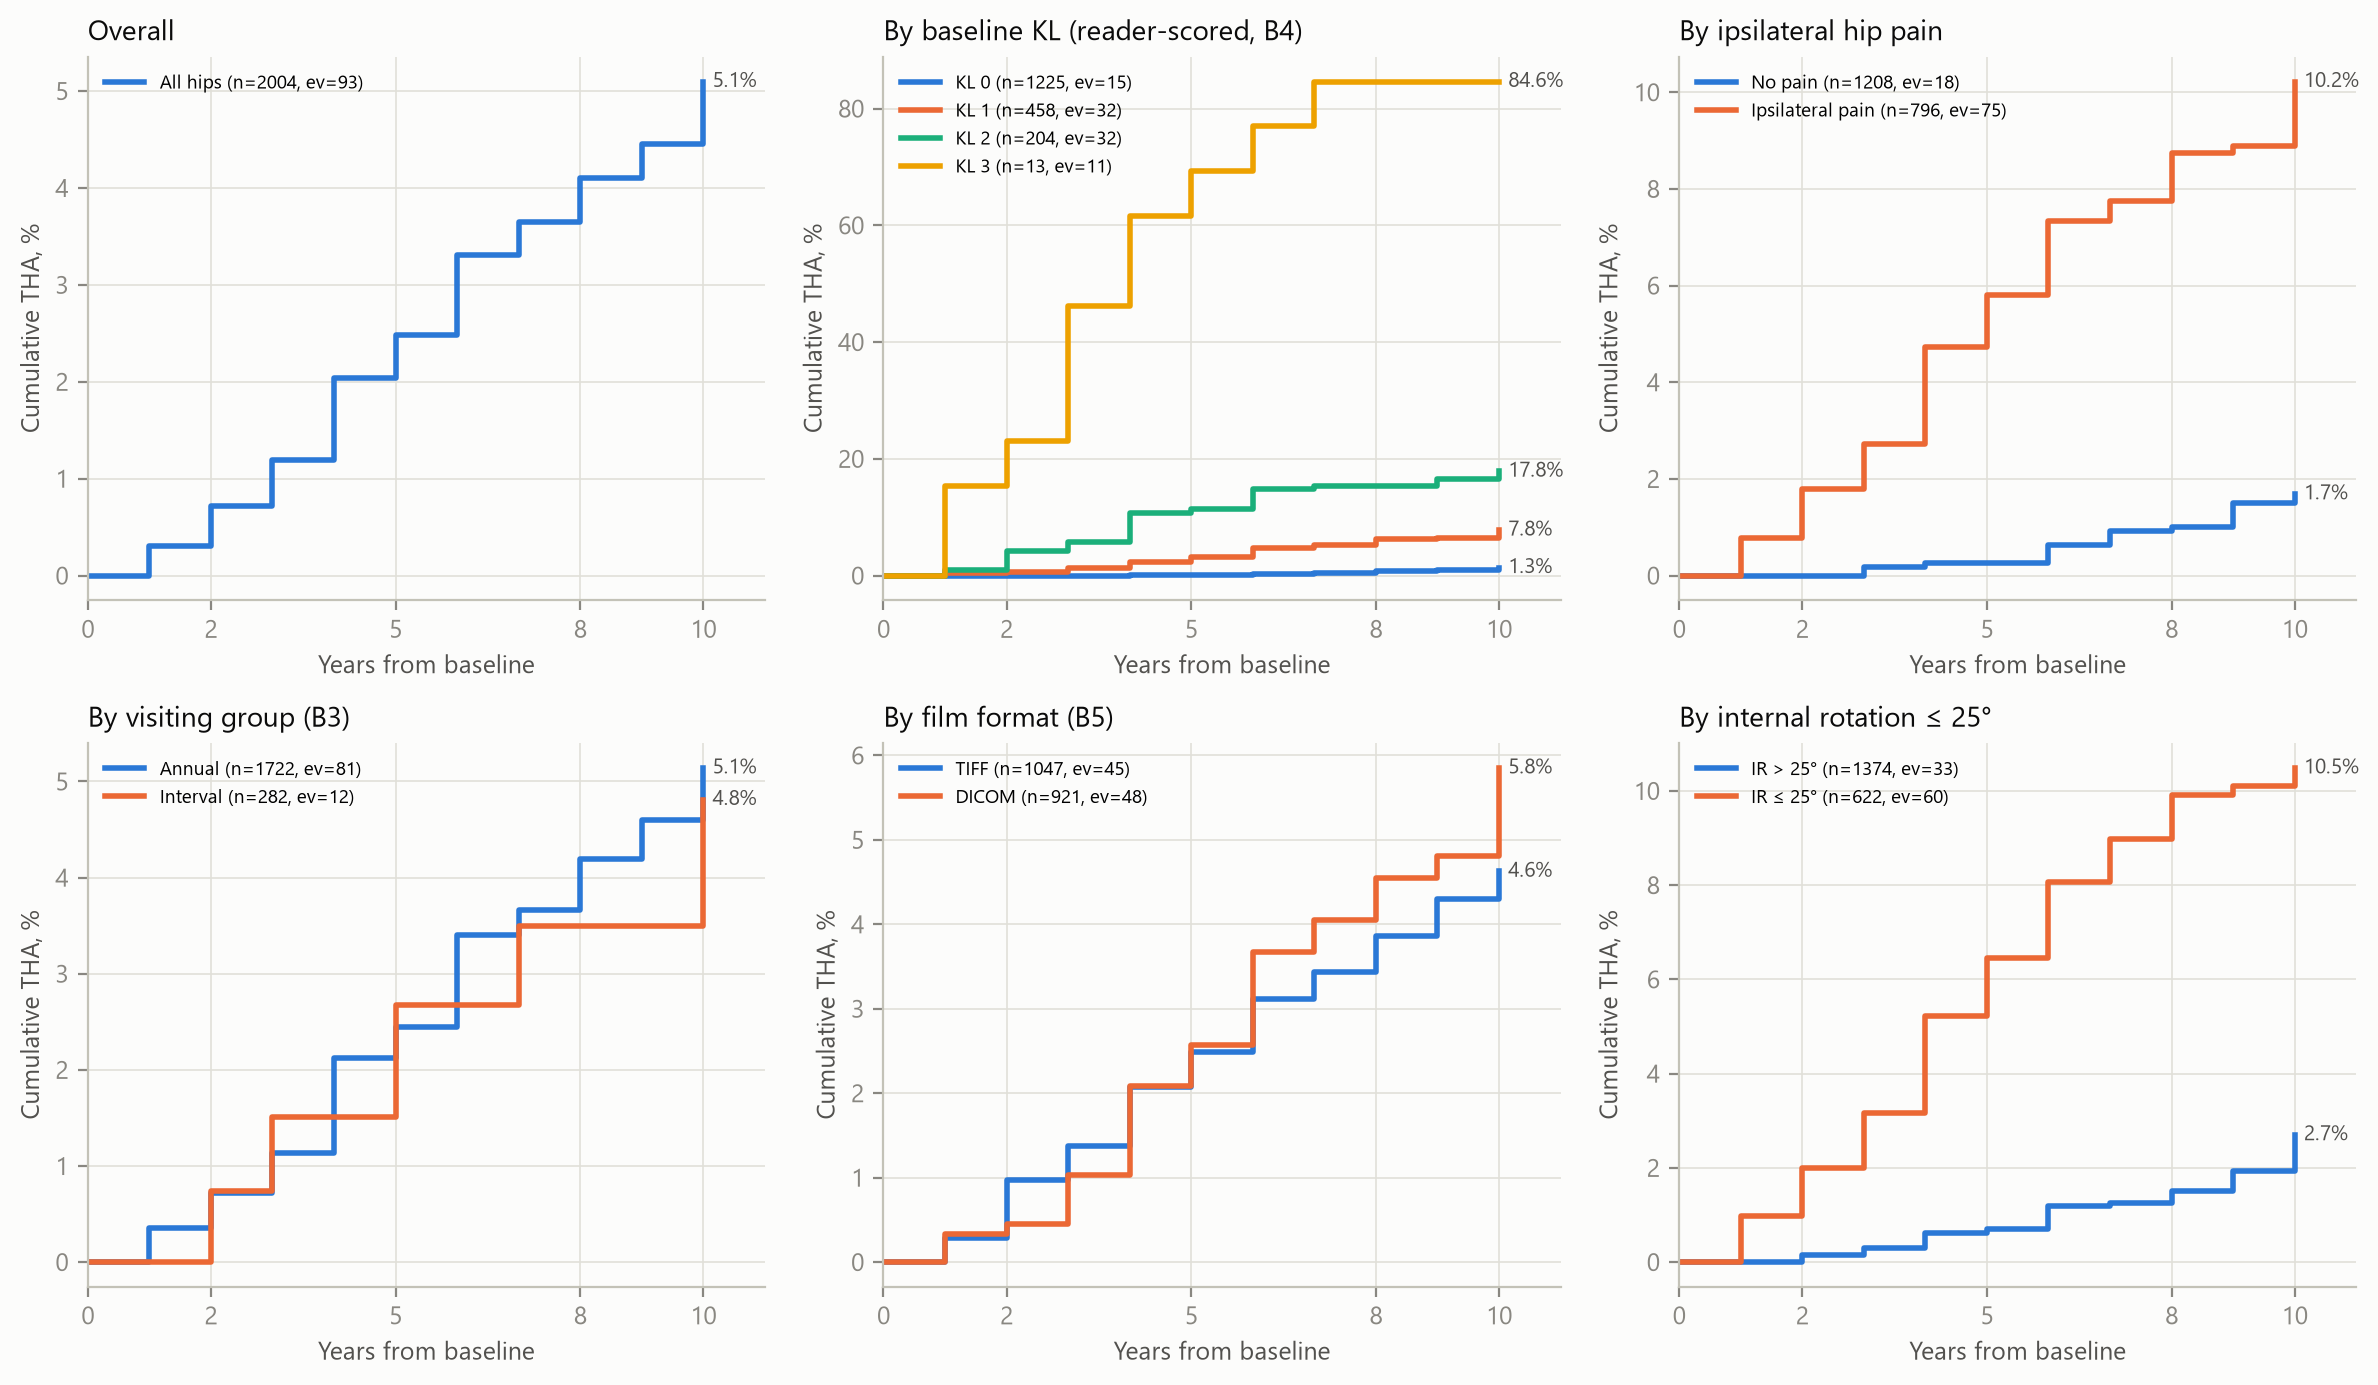
\includegraphics[width=\linewidth]{figS2_km_strata.png}
  \caption{\textbf{Cumulative incidence of THA (Kaplan--Meier) by baseline stratum.} Overall 10-year risk is 5.1\%.
  Ipsilateral hip pain (10.2\% vs 1.7\%) and internal rotation $\le25^\circ$ (10.5\% vs 2.7\%) separate risk
  strongly, whereas visiting group and film format do not. The reader-scored KL panel is shown for description only;
  these readings are not model inputs (Fig.~\ref{fig:timeline}).}
  \label{fig:s-km}
\end{figure}

\begin{figure}[!htbp]
  \centering
  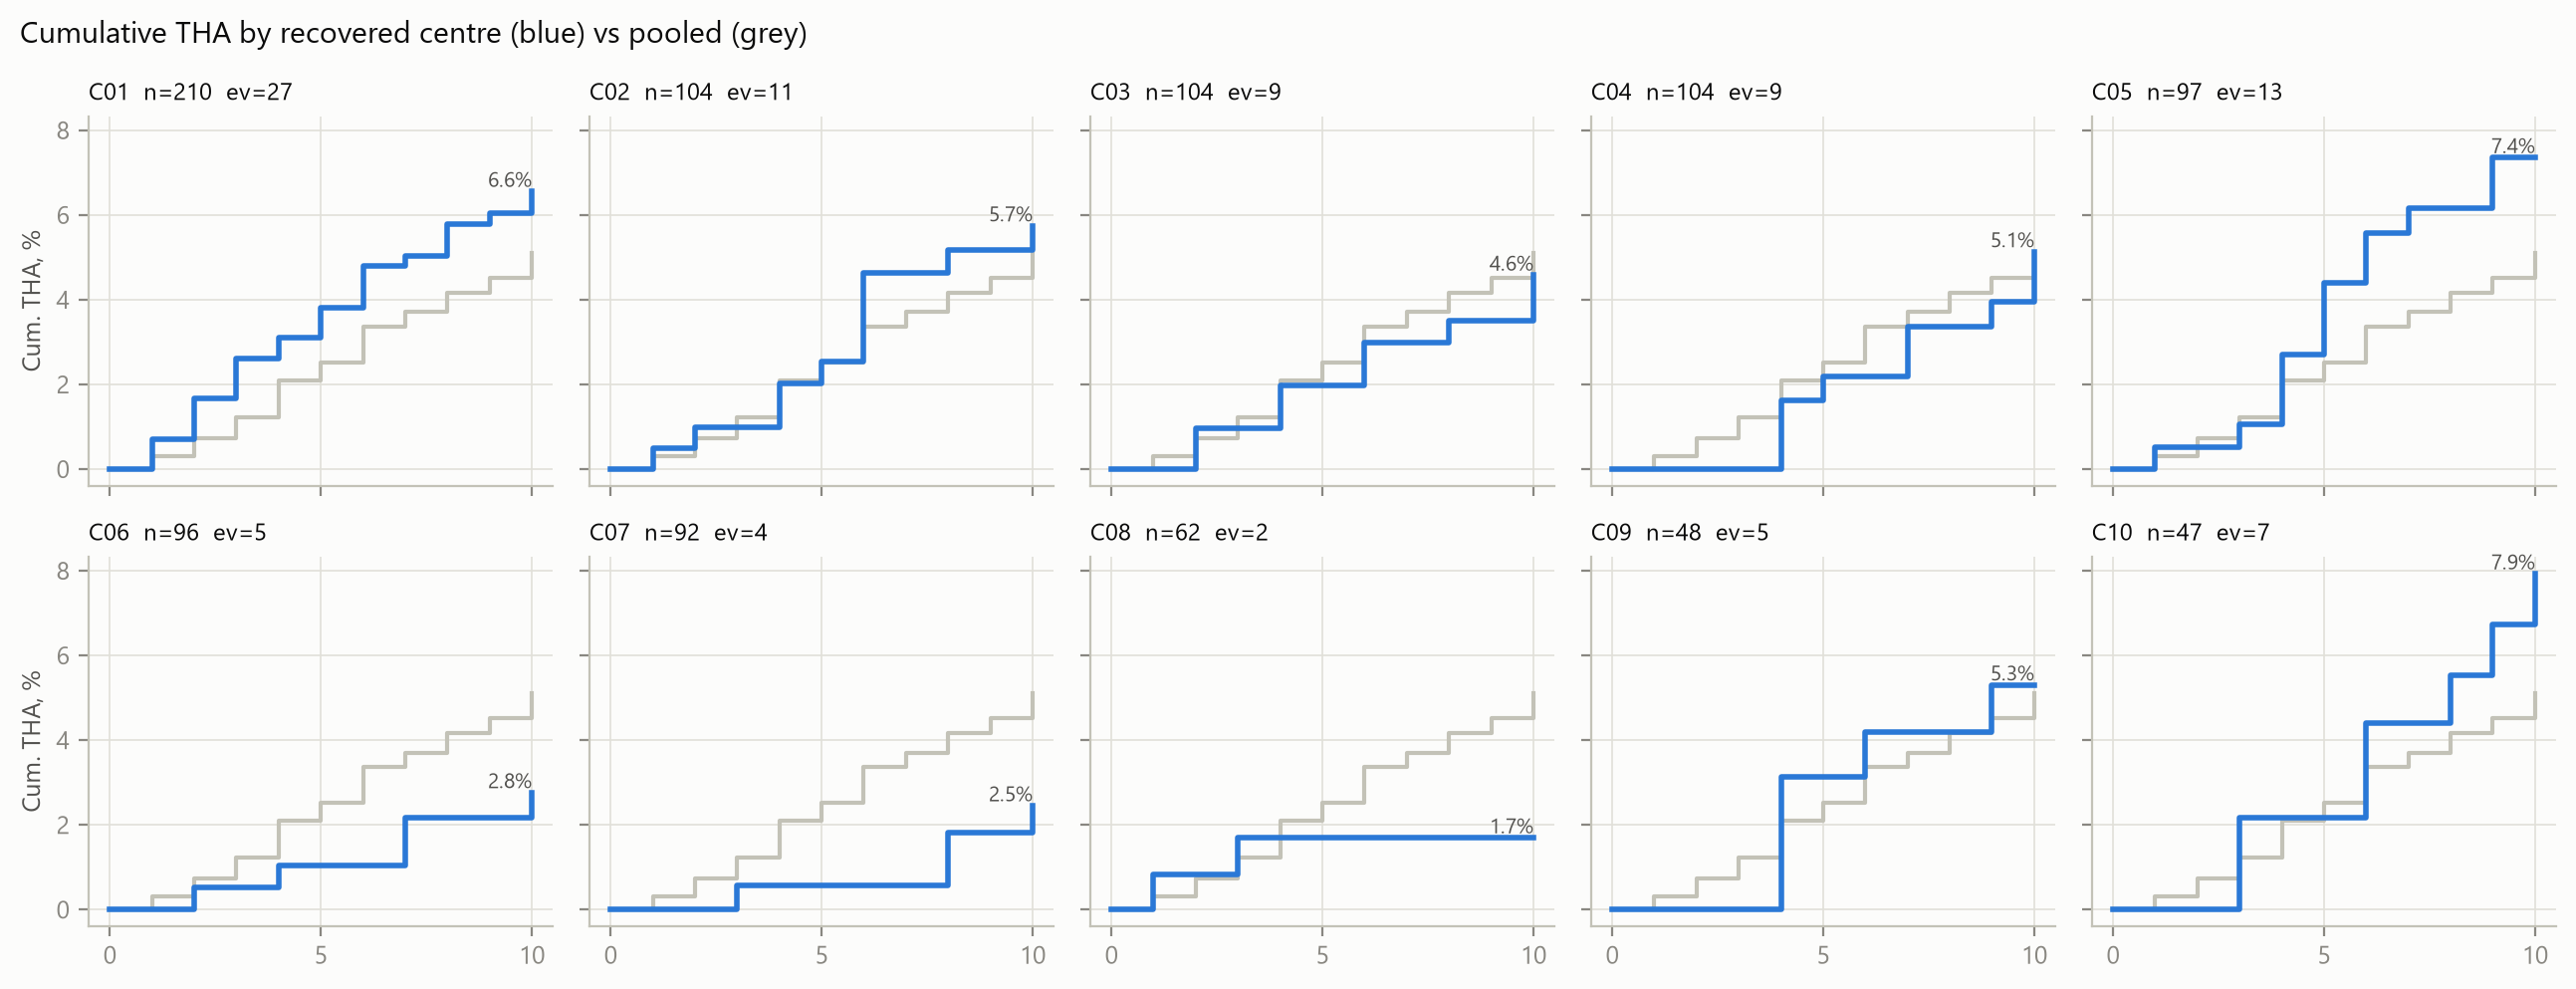
\includegraphics[width=\linewidth]{figS3_km_centre.png}
  \caption{\textbf{Cumulative incidence of THA by recovered centre} (blue) against the pooled curve (grey). Ten-year
  risk ranges from 1.7\% (C08, 2 events) to 7.9\% (C10, 7 events); the centre--outcome association is not significant
  (participant-clustered GEE $p=0.36$). Centre is metadata only, never a model input; it defines the
  leave-one-centre-out transport split.}
  \label{fig:s-km-centre}
\end{figure}

\begin{figure}[!htbp]
  \centering
  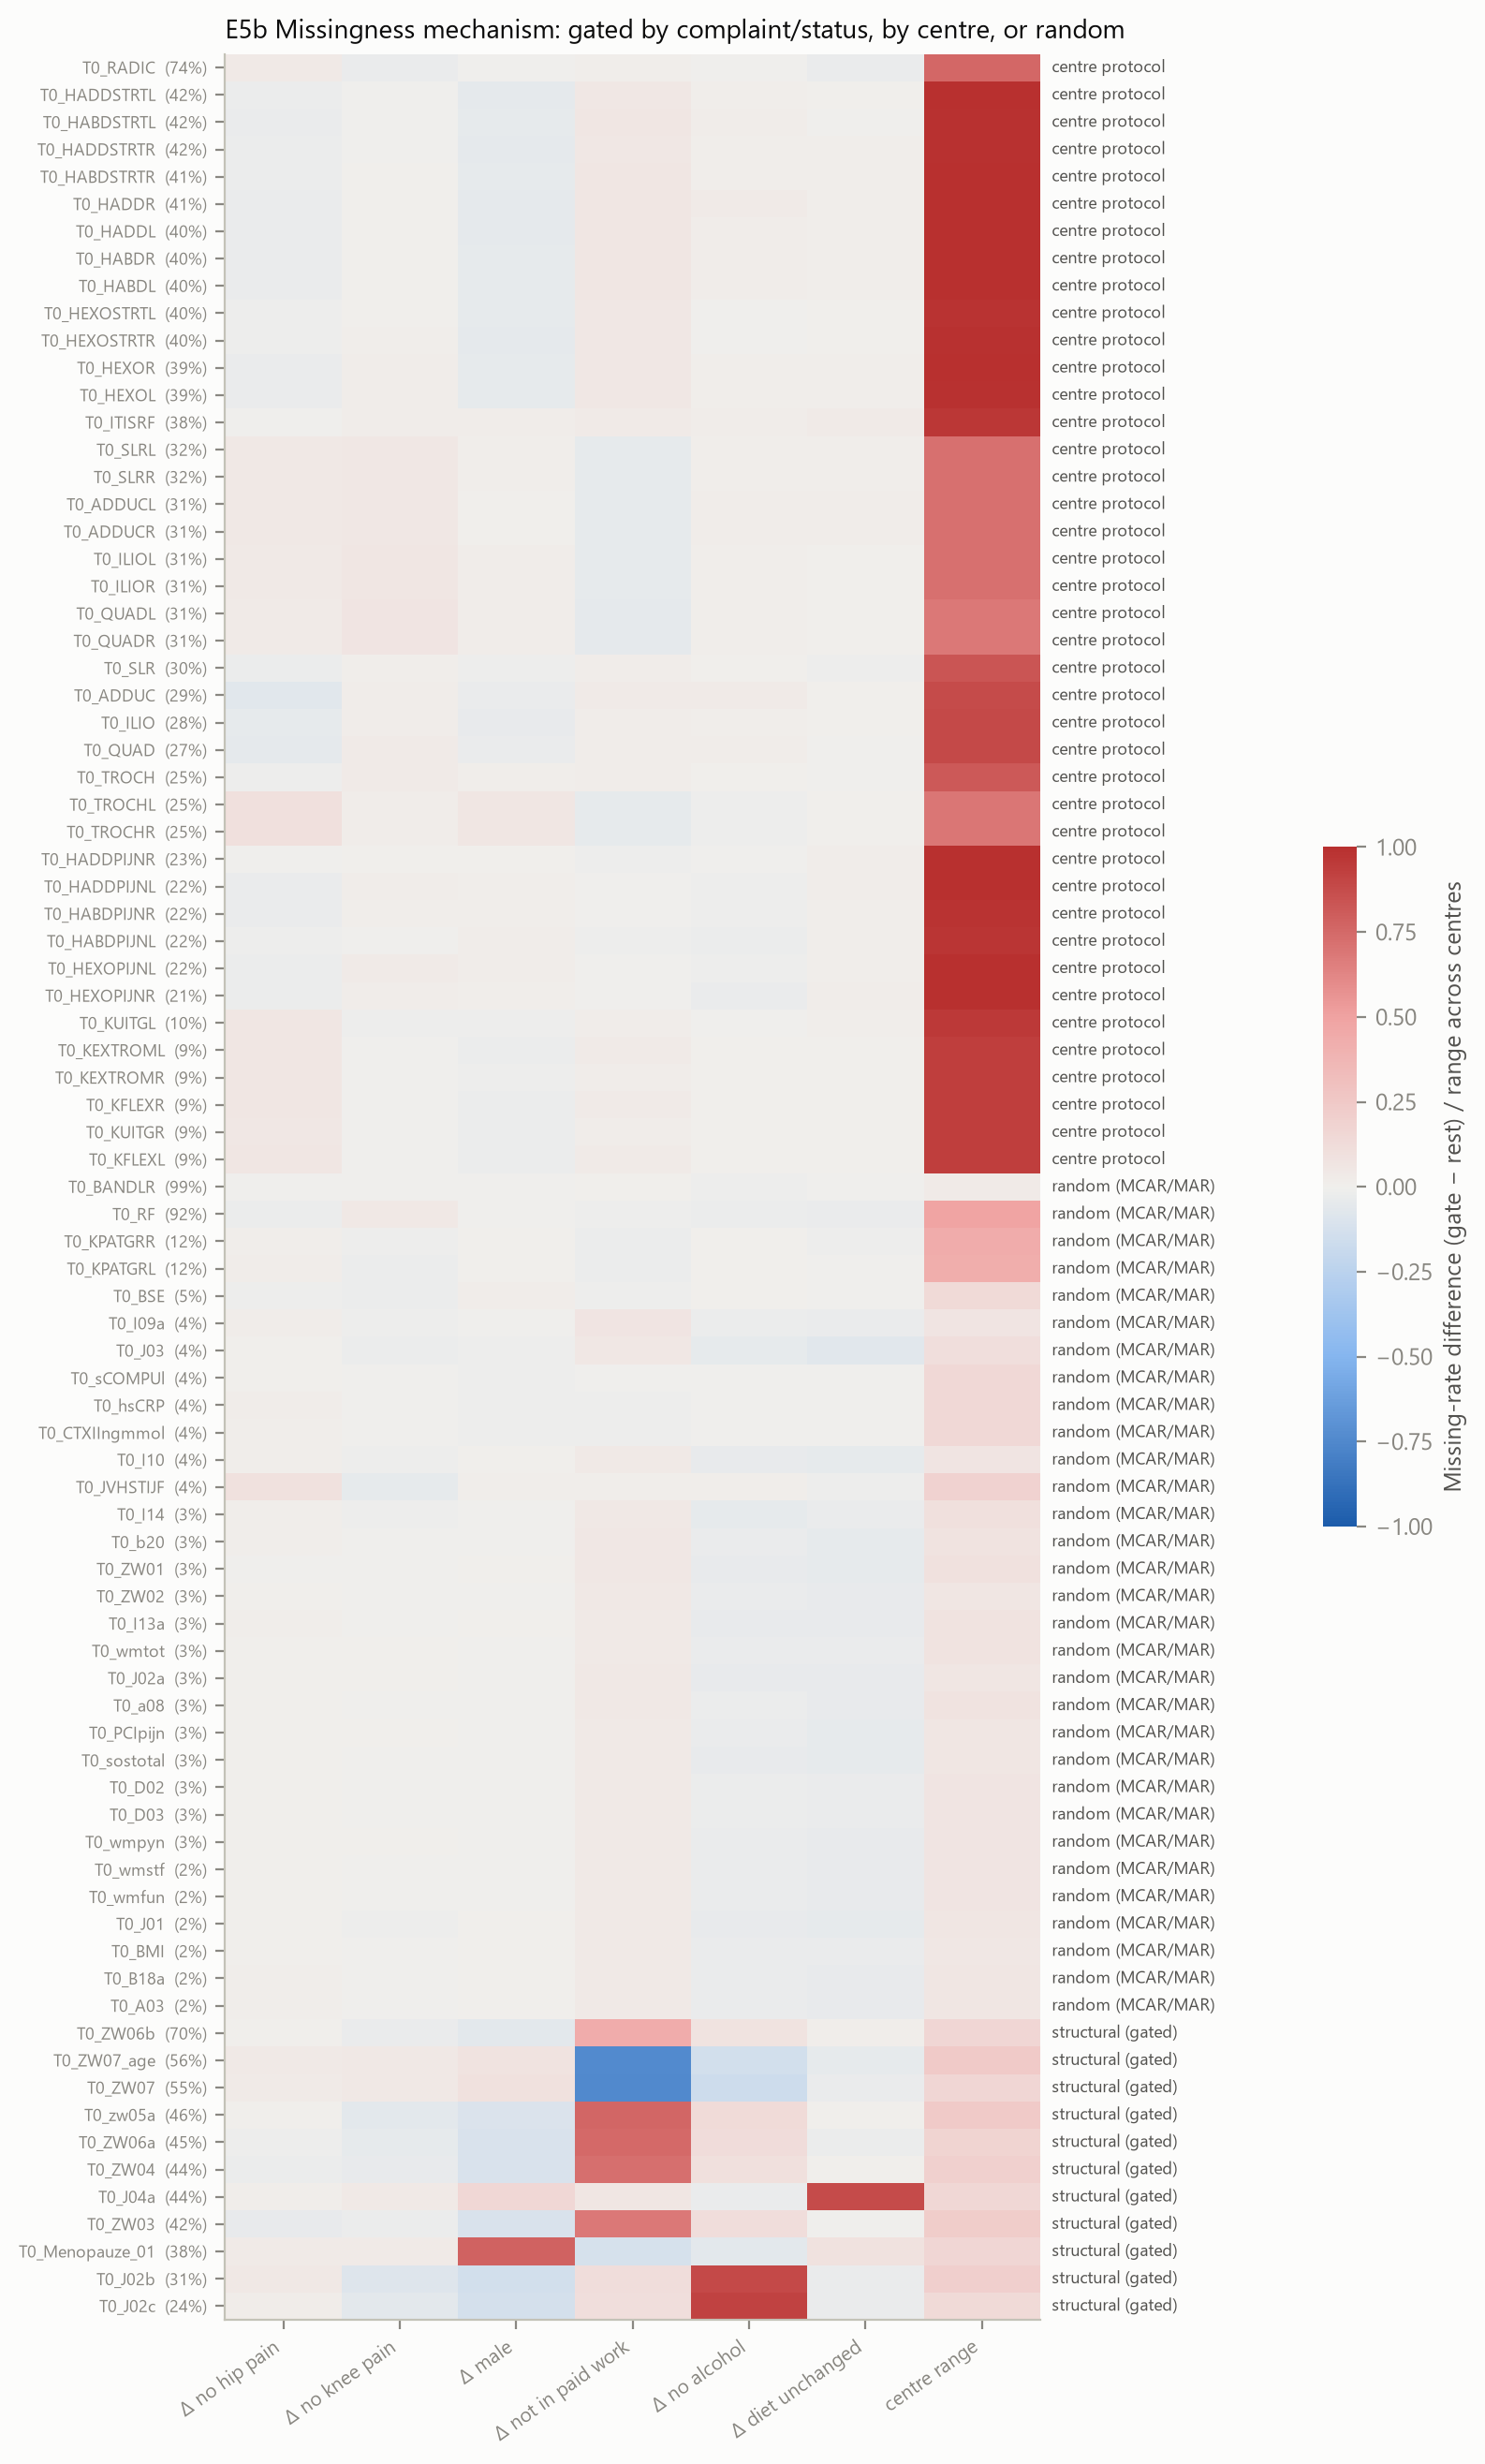
\includegraphics[width=0.82\linewidth]{figS4_missing_mechanism.png}
  \caption{\textbf{Missingness mechanism of every raw variable with $>$2\% missing.} Columns compare the missing rate
  between a gate (no hip pain, no knee pain, male, not in paid work, no alcohol, diet unchanged) and the rest, and give
  the range of missing rates across centres. Variables are classed as centre protocol (41; range near 1, e.g.\ external
  rotation, adduction and abduction ROM), structural / gated (38; coded by questionnaire logic) or sporadic (92; imputed
  fold-wise by MICE with indicators). Section~\ref{sec:methods} gives the rules.}
  \label{fig:s-missing}
\end{figure}

\begin{figure}[!htbp]
  \centering
  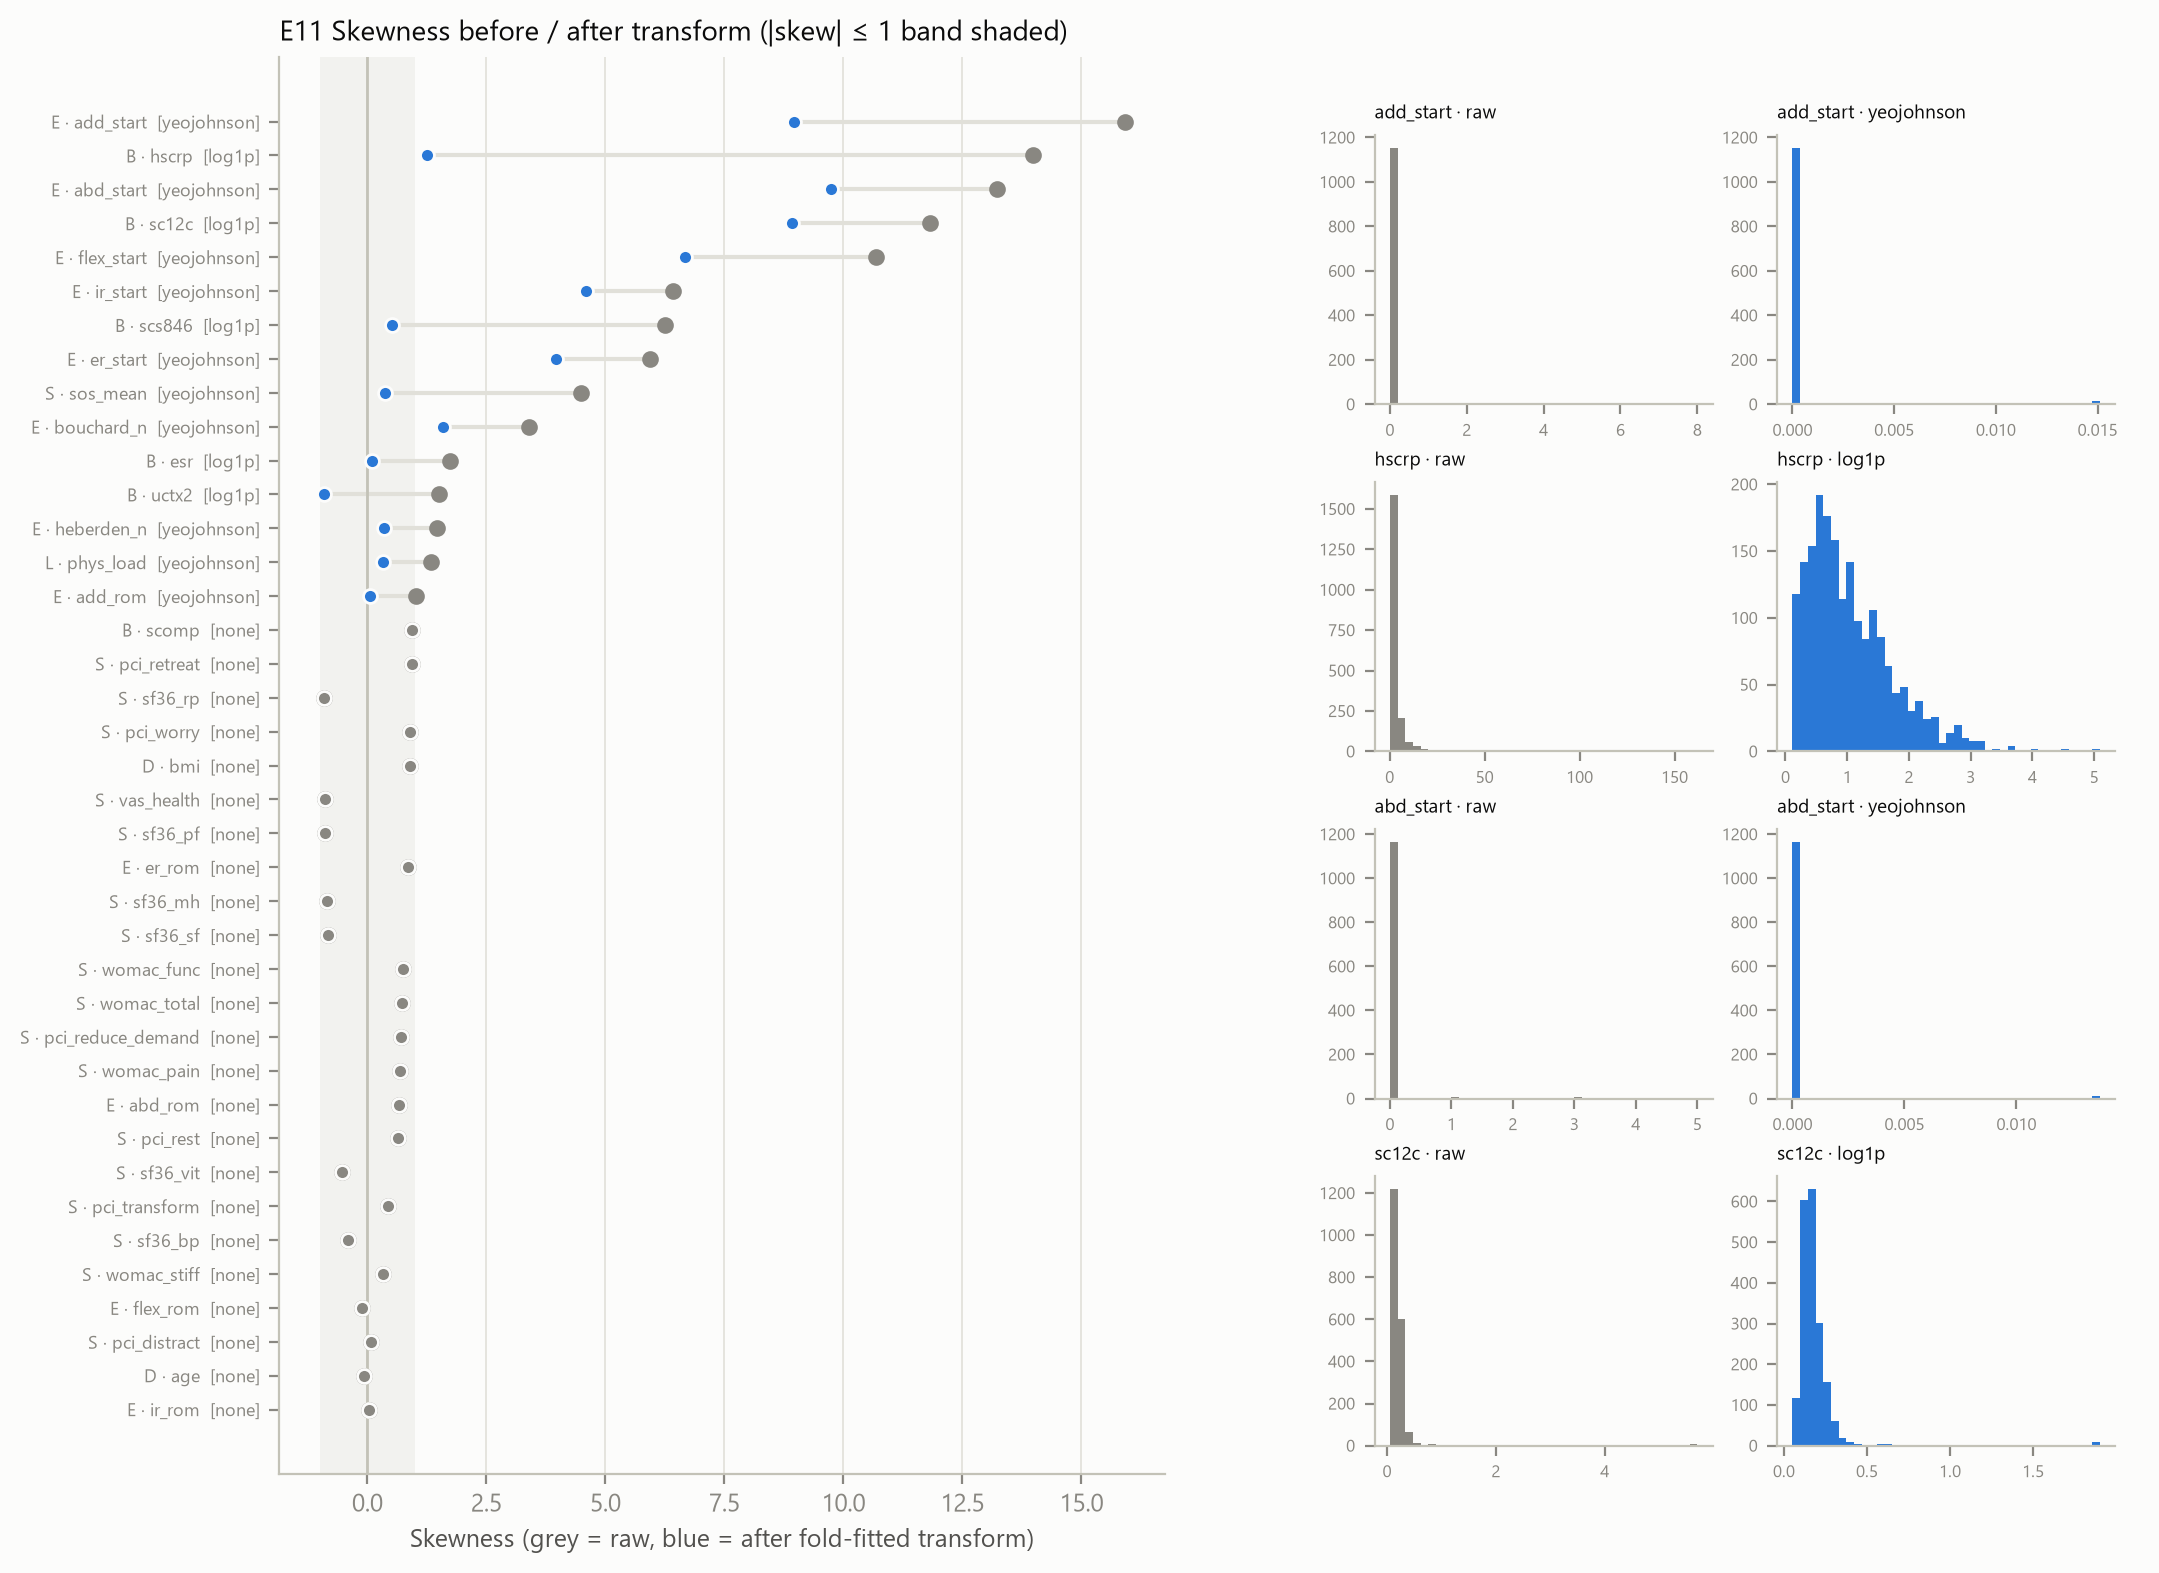
\includegraphics[width=\linewidth]{figS5_skewness.png}
  \caption{\textbf{Skewness before and after the fold-fitted transforms.} Fifteen continuous variables had
  $|\text{skew}|>1$. Biomarkers receive log1p (e.g.\ hsCRP 14 $\to$ 1.2) and other variables Yeo--Johnson, with
  $\lambda$ fitted on training rows, followed by winsorising at the training 0.5/99.5\% quantiles. Variables still
  skewed after transformation are zero-inflated goniometer start positions, which are not in the main set. Right:
  examples of raw and transformed distributions.}
  \label{fig:s-skew}
\end{figure}

\FloatBarrier
\setcounter{figure}{0}
\renewcommand{\thefigure}{A\arabic{figure}}

\section{Pseudo-external transport (full table)}
\label{app:transport}

\begin{table}[!htbp]
  \centering
  \caption{\textbf{Transport of M0 (all clinical features).} The model is trained on source participants, with
  participants who have a hip in the target removed from the source. Platt calibration and the 80\%-sensitivity
  threshold are fitted in the source, and the model is applied unchanged to the target. ``Internal'' is the nested-CV
  out-of-fold performance on the same target hips. $\Delta$ is the paired participant bootstrap (500 draws).}
  \small
  \setlength{\tabcolsep}{3pt}
  \resizebox{\linewidth}{!}{%
  \begin{tabular}{@{}lccccccc@{}}
    \toprule
    Source $\to$ target & Events & AUPRC ext./int. & $\Delta$AUPRC (95\% CI) & AUROC ext./int. & Cal.\ int. & Cal.\ slope & Sens./spec. \\
    \midrule
    Leave-one-centre-out (pooled) & 92 & 0.374 / 0.377 & $-0.003$ ($-0.049$, 0.039) & 0.803 / 0.820 & $-0.10$ & 0.82 & 0.71 / 0.68 \\
    TIFF $\to$ DICOM & 48 & 0.353 / 0.375 & $-0.022$ ($-0.097$, 0.057) & 0.778 / 0.802 & 0.06 & 0.76 & 0.65 / 0.71 \\
    DICOM $\to$ TIFF & 45 & 0.421 / 0.413 & 0.008 ($-0.085$, 0.087) & 0.850 / 0.843 & $-0.41$ & 1.08 & 0.87 / 0.63 \\
    Annual $\to$ interval group & 12 & 0.211 / 0.172 & 0.039 ($-0.019$, 0.157) & 0.799 / 0.788 & 0.30 & 0.74 & 0.75 / 0.67 \\
    Painful $\to$ painless hips & 18 & 0.099 / 0.101 & $-0.001$ ($-0.136$, 0.064) & 0.673 / 0.679 & $-1.47$ & 1.00 & 0.72 / 0.52 \\
    Female $\to$ male & 25 & 0.594 / 0.565 & 0.029 ($-0.060$, 0.100) & 0.903 / 0.902 & 0.28 & 1.39 & 0.92 / 0.62 \\
    High $\to$ low education & 65 & 0.406 / 0.420 & $-0.014$ ($-0.070$, 0.053) & 0.797 / 0.817 & 0.05 & 0.89 & 0.78 / 0.60 \\
    Low $\to$ high education & 26 & 0.318 / 0.365 & $-0.047$ ($-0.188$, 0.084) & 0.810 / 0.823 & $-0.41$ & 0.83 & 0.77 / 0.66 \\
    Prior care $\to$ none & 40 & 0.287 / 0.306 & $-0.018$ ($-0.082$, 0.061) & 0.806 / 0.789 & $-0.47$ & 0.71 & 0.70 / 0.74 \\
    No prior care $\to$ care & 52 & 0.354 / 0.481 & $\mathbf{-0.128}$ ($-0.220$, $-0.028$) & 0.807 / 0.848 & 0.08 & 1.22 & 0.94 / 0.40 \\
    \bottomrule
  \end{tabular}}
\end{table}

Per-centre calibration intercepts ranged from $-1.64$ (C08, 2 events) to $+1.37$ (C10, 7 events).
Image head (residual + OARSI; one fit per split, no bootstrap; internal reference = repeat-0 out-of-fold scores):
leave-one-centre-out AUROC/AUPRC 0.858/0.483 (internal 0.876/0.526); TIFF$\to$DICOM 0.813/0.465 (0.872/0.583);
DICOM$\to$TIFF 0.844/0.369 (0.883/0.495).

\section{Leakage audit of the code}
\label{app:audit}
Every fitted transformation, selection and calibration step was traced to the rows it was fitted on. Three deviations
from strict nesting were found, none of which touches M0 or the final fusion model.
\begin{enumerate}[itemsep=0pt]
  \item NAS stage 1 scored architectures on one outer split (repeat 0, fold 0), which is a test fold in 24 other splits.
        This affects M2 and M4.
  \item The SimCLR checkpoint was selected by a linear probe on the labels of the same split. This affects only the
        SimCLR variants.
  \item The pain and format domains of the transport experiment were first defined per hip, which placed 329
        participants on both sides of the split. This is \textbf{fixed}: the table above uses participant-disjoint
        sources.
\end{enumerate}
Label-free global steps are disclosed in Section~\ref{sec:methods}. The inner selection of the fusion model uses
singly, not doubly, cross-fitted logits; this is a second-order effect on tuning only.

\section{Links to the course lectures}
\label{app:lectures}
Slides refer to the MD6329 lecture PDFs; times refer to the lecture recordings
(\url{https://www.youtube.com/playlist?list=PLORG7zBQosxw}). We list only the points where this study uses or departs
from a technique covered in the course.

\begin{table}[!htbp]
  \centering
  \small
  \setlength{\tabcolsep}{4pt}
  \begin{tabular}{@{}p{0.43\linewidth}p{0.2\linewidth}p{0.13\linewidth}p{0.17\linewidth}@{}}
    \toprule
    Point in this report & Slides & Recording & Section \\
    \midrule
    Frozen ImageNet features as a feature extractor (our first image baseline; Bar et al.) & L02 p.\,102, 126--127 & 1:00--1:05 & Methods M3; Results \\
    How much data deep learning needs; transfer learning, which layers to freeze & L02 p.\,106--114 & 0:54--0:56 & Methods M3; Limitation 1 \\
    DenseNet-121 on radiographs (CheXNet) and saliency maps & L02 p.\,158; L11 p.\,34--35 & 1:29--1:31 & Methods M3; Fig.~\ref{fig:attention} \\
    Precision--recall for imbalanced data (AUPRC as primary metric) & L02 p.\,95 & -- & Results \\
    Class-weighted loss for imbalance (inverse class frequency; our pos\_weight) & L03 p.\,63--64 & 0:31--0:34 & Methods \\
    Dice and Jaccard overlap (our locator evaluation) & L03 p.\,65 & -- & Results \\
    Early / joint / late fusion (our token, FiLM and logit fusion) & L08 p.\,30 & 0:11--0:14 & Methods; Discussion \\
    Self-supervised learning, SimCLR & L08 p.\,42--50 & 0:17--0:20 & Methods; Results \\
    Attention as interpretability & L11 p.\,5 & -- & Results \\
    Occlusion, saliency, CAM (our attention maps) & L11 p.\,15--33 & 0:15--0:24 & Results \\
    Is model confidence trustworthy? (calibration) & L11 p.\,40 & 0:28--0:33 & Results \\
    Performance differences across populations (transport splits) & L11 p.\,45 & 0:28--0:33 & Results \\
    \bottomrule
  \end{tabular}
\end{table}

\section{Software 3.0 statement}
An AI coding agent (Claude Opus 5.5, used through Claude Code) took part in problem formulation, coding and evaluation.
Every suggestion was checked against the data, the code or the source paper before it was used, and several were rejected
or changed (below).

\paragraph{What the AI did.}
\begin{itemize}[leftmargin=*,itemsep=1pt]
  \item \emph{Problem formulation and literature.} It ran scripted searches of the Europe PMC API (six query families, 208
        unique records, 49 abstracts read in full) and tabulated cohorts, endpoints and metrics (Table~\ref{tab:forest}).
        It also wrote the feasibility analysis: data access per candidate dataset, the size of the imaging work, and
        benchmark-based estimates of training time for each model on a CPU-only laptop.
  \item \emph{Image data curation.} It found that about 110 films were stored rotated by $90^\circ$ and built the
        self-supervised rotation fix. It also redesigned the femoral-head locator's decoding, which cut gross errors from
        19\% to 1.8\%.
  \item \emph{Model engineering and audit.} It wrote most of the pipeline code. It found that the discrete-time head
        never trained (zero-initialised hazard bias). It traced M2's instability to early stopping on about 25 noisy
        validation events, using the per-repeat SD and the distribution of stopping epochs. It audited the code line by
        line for train/test leakage (Appendix~\ref{app:audit}), which led to the participant-disjoint transport splits.
  \item \emph{Interpretation and writing support.} It drafted the interpretation of part of the experimental results,
        produced the data-driven figures, and proofread the report.
\end{itemize}

\paragraph{What the author did.}
\begin{itemize}[leftmargin=*,itemsep=1pt]
  \item \emph{Topic and question.} Chose CHECK after weighing dataset accessibility. Defined the clinical problem: 10-year ipsilateral THA as the endpoint instead of radiographic OA, rare
        events treated as a feature of the problem, and first presentation as the prediction time.
  \item \emph{Features and design.} Selected the feature groups and the redundancy and missingness rules. Designed the
        experiments: nested repeated grouped CV instead of a 20\% hold-out, no SMOTE, leave-one-centre-out as the main
        transport split, and no language model.
  \item \emph{Architecture.} Chose and optimised the architectures: SimCLR with forgetting guards, the dual-head
        FT-Transformer, and the decision to supervise the image branch after its first version underperformed.
  \item \emph{Validity checks.} Rejected label permutation and KL stratification as sufficient evidence against leakage
        and required the temporal audit, which defined the admissibility of every input at $t_0$.
  \item \emph{Analysis and writing.} Designed the auxiliary analyses and analysed their results. Wrote the narrative
        logic and most of the content of this report.
\end{itemize}

\paragraph{Effect on the workflow.} The agent made exhaustive checks cheap: line-by-line leakage tracing, rerunning all
five repeats, verifying literature numbers against full texts. It also exposed errors that a single pass would have
missed, such as the rotated films, the untrained head and the hip-level transport split. Its own suggestions also needed
correcting. It initially proposed using the OARSI items as auxiliary targets, then withdrew the idea as leakage-prone; it
was later reinstated as targets only, after the temporal audit. Every number in the report was regenerated from saved
out-of-fold predictions by scripts in the supplementary material and the code repository (\url{\repourl}).


\end{document}
